\documentclass[aspectratio=1610]{beamer}

%%{ header

\mode<presentation> {

  %%{ themes

  % \usetheme{default}
  % \usetheme{annarbor}
  % \usetheme{antibes}
  % \usetheme{bergen}
  % \usetheme{berkeley}
  % \usetheme{berlin}
  % \usetheme{boadilla}
  % \usetheme{cambridgeus}
  % \usetheme{copenhagen}
  % \usetheme{darmstadt}
  % \usetheme{dresden}
  % \usetheme{frankfurt}
  % \usetheme{goettingen}
  % \usetheme{hannover}
  % \usetheme{ilmenau}
  % \usetheme{juanlespins}
  % \usetheme{luebeck}
  % \usetheme{madrid}
  % \usetheme{malmoe}
  % \usetheme{marburg}
  % \usetheme{montpellier}
  % \usetheme{paloalto}
  % \usetheme{pittsburgh}
  % \usetheme{rochester}
  % \usetheme{singapore}
  % \usetheme{szeged}
  % \usetheme{warsaw}
  % \usetheme{dbt}
  % \usetheme{ClassyCharcoal}
  \usetheme{Boadilla}

  %%}

  %%{ color themes

  % \usecolortheme{albatross}
  % \usecolortheme{beaver}
  % \usecolortheme{beetle}
  % \usecolortheme{crane}
  % \usecolortheme{dolphin}
  % \usecolortheme{dove}
  % \usecolortheme{fly}
  % \usecolortheme{lily}
  % \usecolortheme{orchid}
  % \usecolortheme{rose}
  % \usecolortheme{seagull}
  % \usecolortheme{seahorse}
  % \usecolortheme{whale}
  % \usecolortheme{wolverine}
  \usecolortheme{seahorse}

  %%}

  % \setbeamertemplate{footline} % remove the footer line
  \setbeamertemplate{footline}[page number] % replace the footer line with simple numbers

  \setbeamertemplate{navigation symbols}{} % removing the navigation symbols

  \setbeamertemplate{section in toc}[square] % change the style of entries in the tableofcontents
  \setbeamertemplate{subsection in toc}[square] % change the style of entries in the tableofcontents
  }

  \usepackage{graphicx} % allows including images
  \usepackage{booktabs} % allows the use of \toprule, \midrule and \bottomrule in tables
  \usepackage{multimedia}
  \newcommand{\superfill}{\vskip0pt plus 1filll}

  \usepackage{tikz}
  \usepackage{pgfplots}
  \usepackage{booktabs} % Allows the use of \toprule, \midrule and \bottomrule in tables
  \usepackage{isotope}
  \usepackage{transparent} % typesetting units
  \usepackage{animate}
  \usepackage{adjustbox}
  \usepackage{subcaption}
  \usepackage{float}
  \usepackage{listings}

  %%{ custom macros

  \newcommand{\unit}[2]{$#1~\ensuremath{\mathrm{#2}}$}
  \newcommand{\strong}[1]{\textbf{#1}}
  \newcommand{\coord}[1]{\textbf{#1}}
  \newcommand{\norm}[1]{\left\lvert#1\right\rvert}
  \newcommand{\m}[1]{\ensuremath{\mathbf{#1}}}
  \newcommand{\edn}[1]{{\color{blue} \textbf{#1}}}
  \newcommand{\todo}[1]{\color{red}{#1}\color{black}}
  \newcommand{\minus}{\scalebox{0.75}[1.0]{$-$}}
  \newcommand{\plus}{\scalebox{0.8}[0.8]{$+$}}

  %%}

  \usetikzlibrary{shapes.arrows,backgrounds,arrows,automata,shapes,positioning,calc,through}

%%{ ARROWS

\tikzset{
  myarrow/.style={
    draw,
    fill=orange,
    single arrow,
    minimum height=3.5ex,
    single arrow head extend=1ex
  }
}

\newcommand{\arrowup}{%
  \vspace{-0.8em}
  \tikz [baseline=-0.5ex]{\node [myarrow,rotate=90] {};}
  \vspace{-1.4em}
}

\newcommand{\arrowdown}{%
  \vspace{-0.8em}
  \tikz [baseline=-1ex]{\node [myarrow,rotate=-90] {};}
  \vspace{-1.5em}
}

\newcommand{\arrowright}{%
  \tikz [baseline=-1ex]{\node [myarrow,rotate=0] {};}
}

\newcommand{\arrowleft}{%
  \tikz [baseline=-1ex]{\node [myarrow,rotate=180] {};}
}

%%}

%%{ CHECKMARK

\def\checkmark{\tikz\fill[scale=0.4](0,.35) -- (.25,0) -- (1,.7) -- (.25,.15) -- cycle;}

%%}

\pgfdeclarelayer{background}
\pgfdeclarelayer{foreground}
\pgfsetlayers{background,main,foreground}

\tikzset{
  state/.style={
    rectangle,
    draw=black, very thick,
    minimum height=1.0em,
    text centered,
  },
  state_gray/.style={
    rectangle,
    draw=black, very thick,
    fill=gray!40,
    minimum height=1.0em,
    text centered,
  },
  state_white/.style={
    rectangle,
    draw=black, very thick,
    fill=white,
    minimum height=1.0em,
    text centered,
    text=black,
  },
  state_green/.style={
    rectangle,
    draw=black, very thick,
    fill=green!50,
    minimum height=1.0em,
    text centered,
    text=black,
  },
  state_red/.style={
    rectangle,
    draw=black, very thick,
    fill=red!70,
    minimum height=1.0em,
    text centered,
    text=black,
  },
  state_blue/.style={
    rectangle,
    draw=black, very thick,
    fill=blue!40,
    minimum height=1.0em,
    text centered,
    text=black,
  },
  final_state/.style={
    rectangle,
    rounded corners,
    draw=black, very thick,
    minimum height=2em,
    text centered,
  },
  initial_state/.style={
    rectangle,
    double=white,
    double distance=1pt,
    inner sep=2pt,
    draw=black, very thick,
    minimum height=2em,
    text centered,
  },
  point/.style={
    circle,
    inner sep=0pt,
    minimum size=3pt,
    fill=red
  },
  nothing/.style={
    rectangle,
    rounded corners,
    draw=white, very thick,
    minimum height=2em,
    inner sep=2pt,
    text centered,
  },
  }



  \logo{\pgfputat{\pgfxy(0,5)}{\pgfbox[right,base]{\includegraphics[height=0.8cm]{}}}}
  \newcommand{\nologo}{\setbeamertemplate{logo}{}}

  \usepackage{eso-pic}
  \newcommand\AtPagemyUpperLeft[1]{\AtPageLowerLeft{\put(\LenToUnit{0.66\paperwidth},\LenToUnit{0.904\paperheight}){#1}}}
  \AddToShipoutPictureFG{
    \AtPagemyUpperLeft{{
\includegraphics[height=0.85cm,keepaspectratio]{fig/logo_ctu_fee_mrs_blue.png}}}
  }
  % \newcommand{\AddToShipoutPictureFG}{\setbeamertemplate{logo}{}}

  %%}

  %%{ TITLE PAGE

  \title[]{Introduction to the Unmanned Aerial Platform in the MRS Lab \\ \small{From control theory to practical experiments}}

  \author[Tomas Baca]{Tomas Baca$^1$, Petr Stibinger$^1$, Robert Penicka$^1$}
  \institute[CTU in Prague]
  {
    \\
    \vspace{1em}
    \begin{tiny}
      $^1$Multi-Robot Systems group, Faculty of Electrical Engineering\\
      Czech Technical University in Prague\\
    \end{tiny}
    \medskip
    \textit{tomas.baca@fel.cvut.cz}
  }
  \date{}

  \titlegraphic{
\includegraphics[width=5cm]{./fig/logo_ctu_fee_mrs_blue.png}}

  \begin{document}

  \begin{frame}
    \titlepage % Print the title page as the first slide
  \end{frame}

  % % todo pix its placement on every page
  % \logo{%
  %   \makebox[1.0\textwidth]{%
  %     \hfill%
  %     
\includegraphics[width=3.0cm, keepaspectratio]{fig/logo_ctu_fee_mrs_blue.png}\vspace{-200pt}
  %   }
  % }

  % \nologo

  %%}

  %%{ TABLE OF CONTENTS

  \begin{frame}
    \frametitle{Outline}
    \tableofcontents
  \end{frame}

  %%}

  %% --------------------------------------------------------------
  %% |                 UAV Experimentation in MRS                 |
  %% --------------------------------------------------------------

  %%{ UAV Experimentation in MRS

  \section{UAV Experimentation in MRS}

  \begin{frame}
    \frametitle{UAV Experimentation in MRS --- 2012--2015}

    \only<+>{\begin{block}{$\approx$ 2012, designing custom PCBs for controllers}
      \begin{figure}
        \centering
        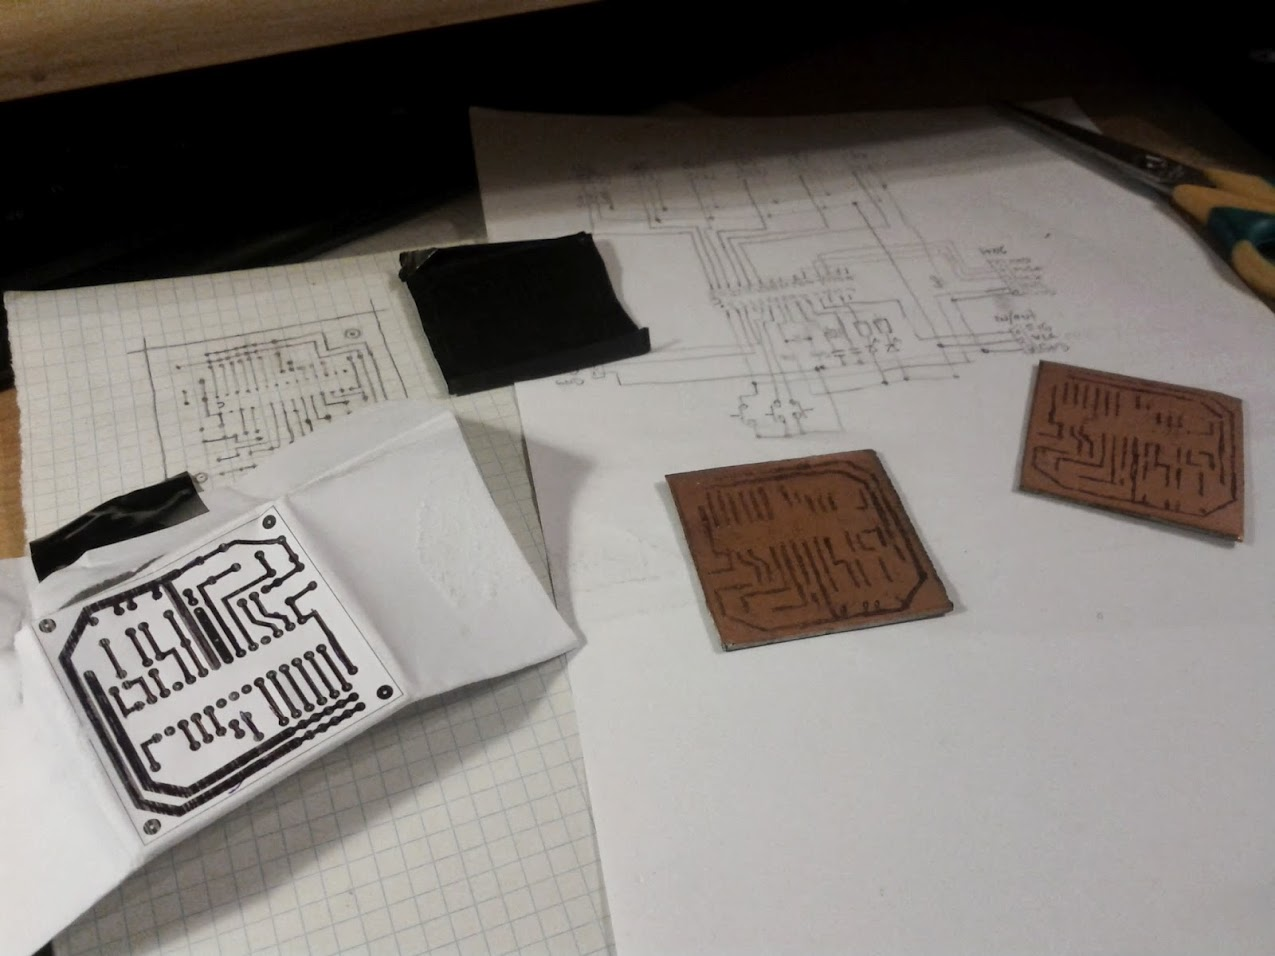
\includegraphics[width=0.60\textwidth]{fig/pcb1.jpg}
      \end{figure}
    \end{block}}

    \only<+>{\begin{block}{$\approx$ 2014, Model Predictive Control on embedded hardware}
      \begin{figure}
        \centering
        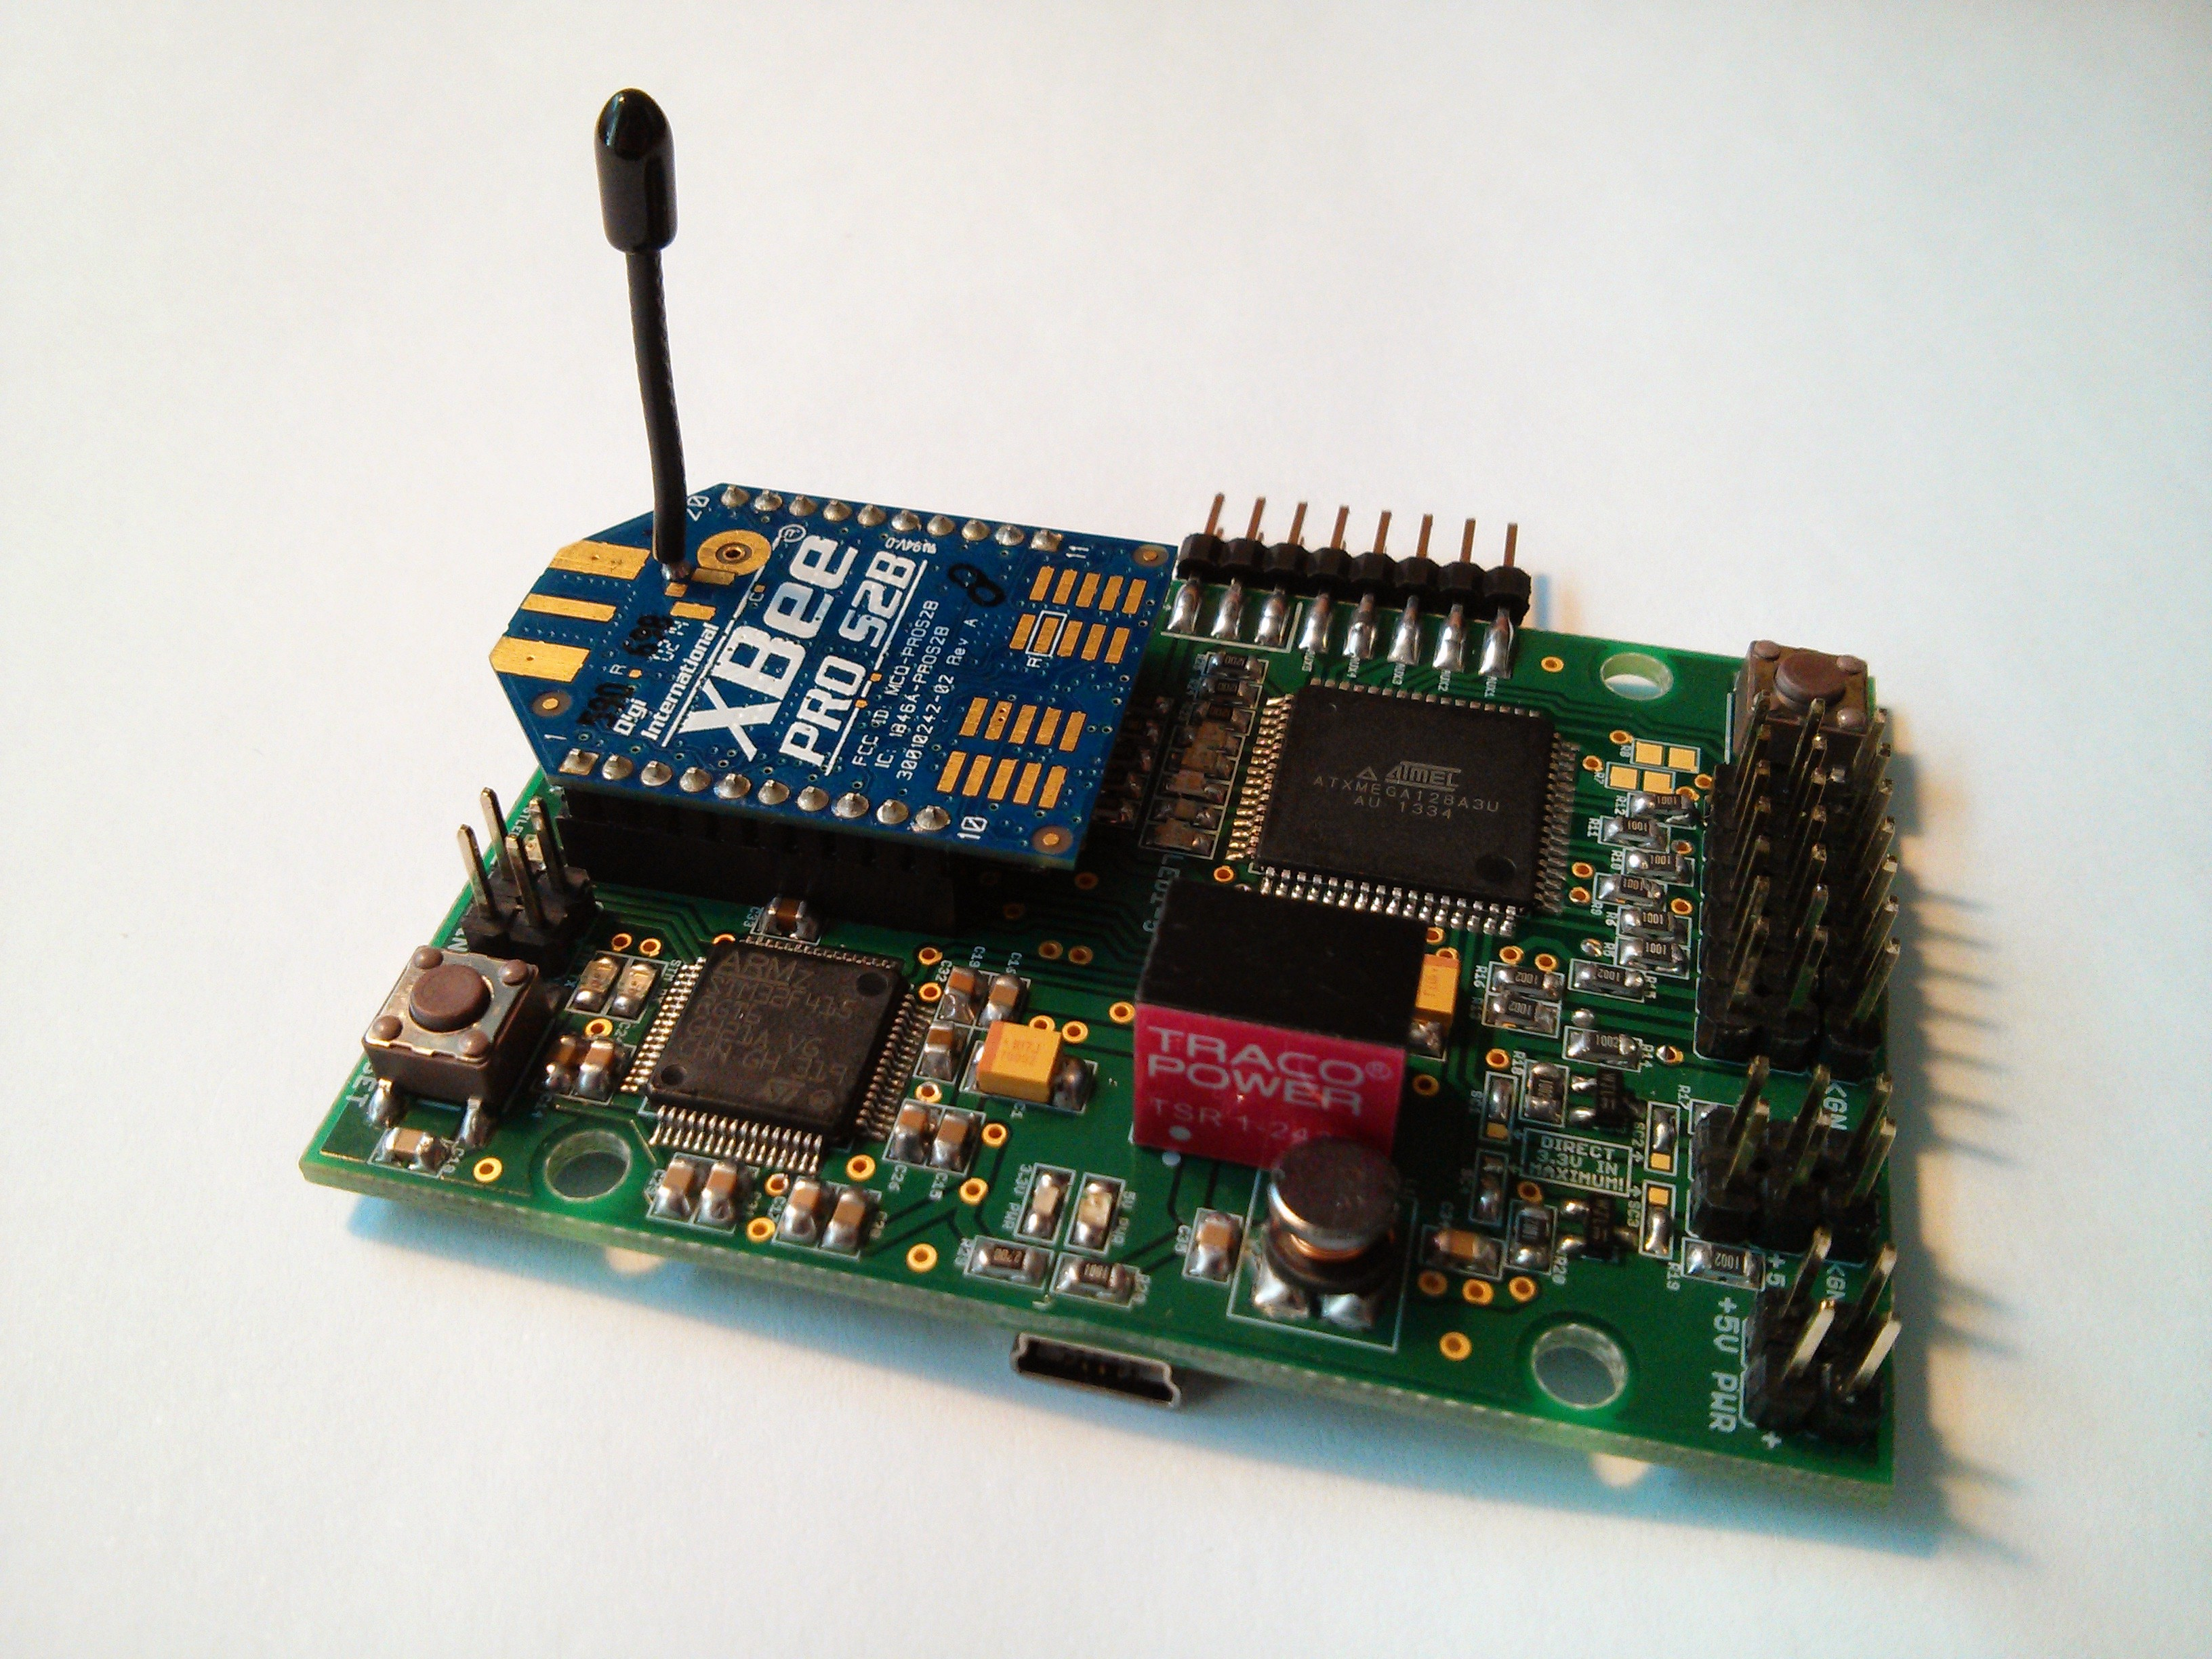
\includegraphics[width=0.60\textwidth]{fig/pcb2.jpg}
      \end{figure}
    \end{block}}

    \only<+>{\begin{block}{$\approx$ 2014, Model Predictive Control on embedded hardware}
      \begin{figure}
        \centering
        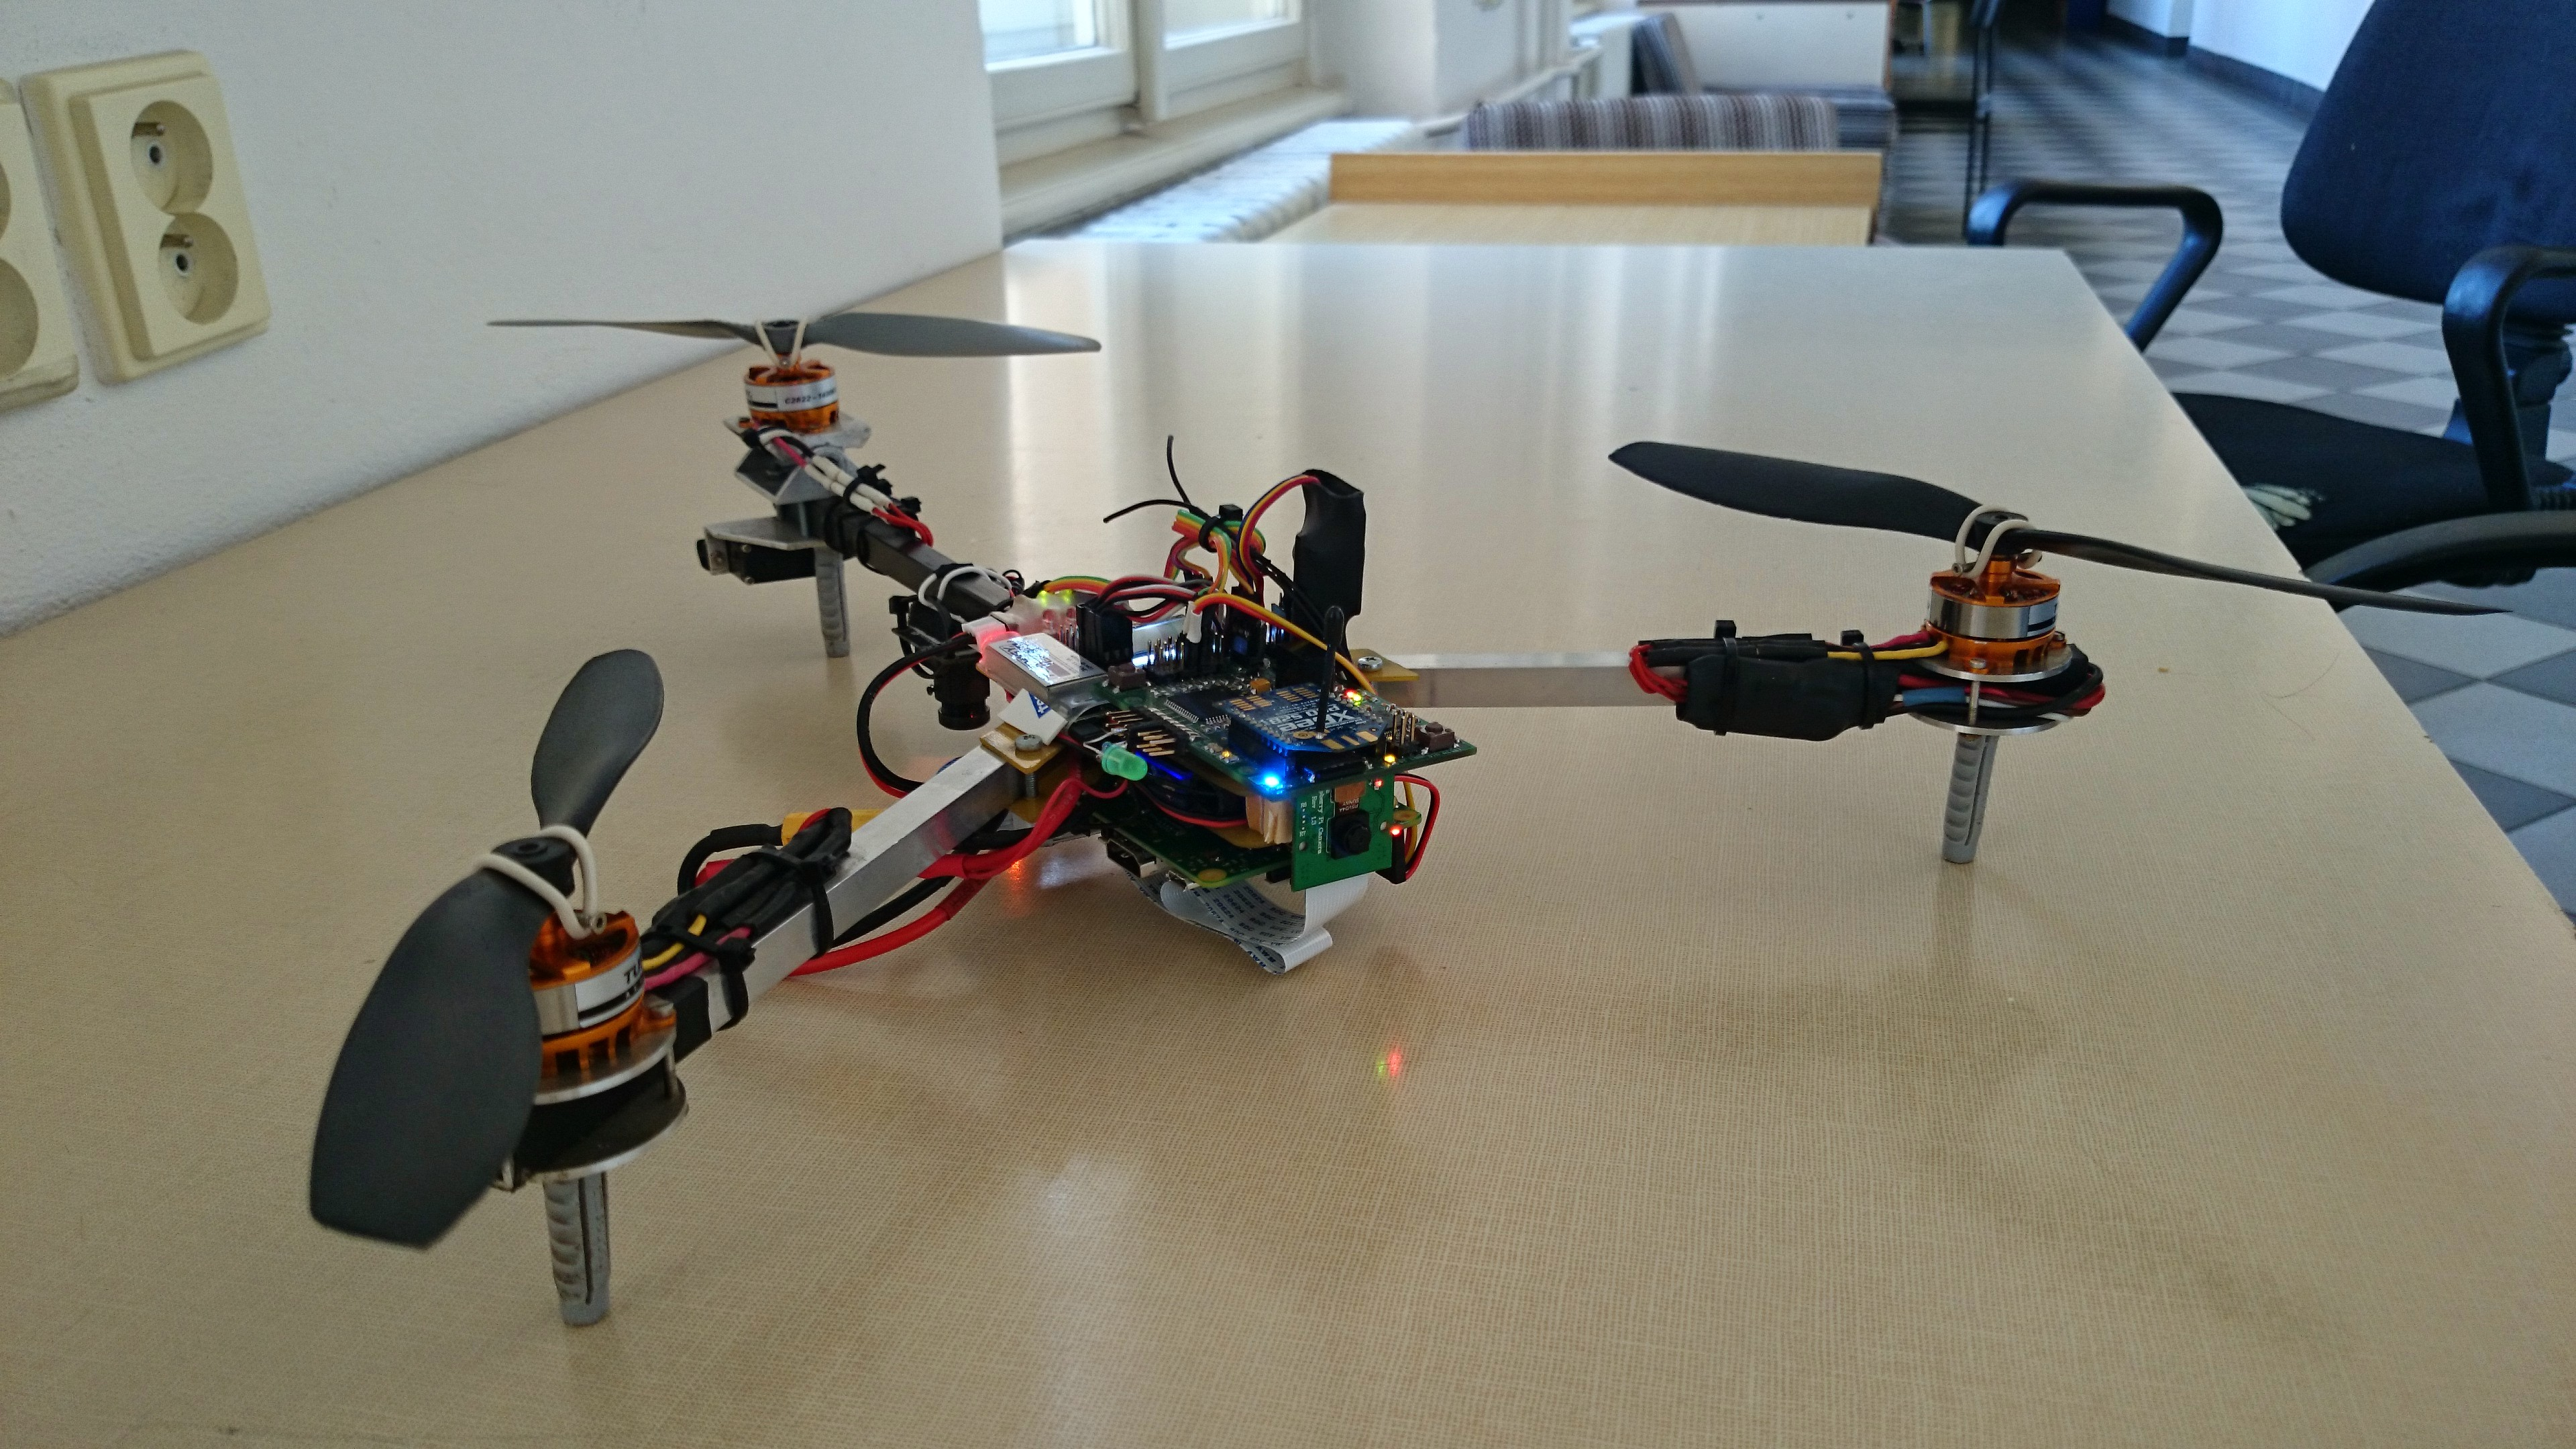
\includegraphics[width=0.90\textwidth]{fig/tricopter.jpg}
      \end{figure}
    \end{block}}

    \only<+>{\begin{block}{Embedded Model Predictive Control}
      \begin{center}

        \movie[autostart]{
          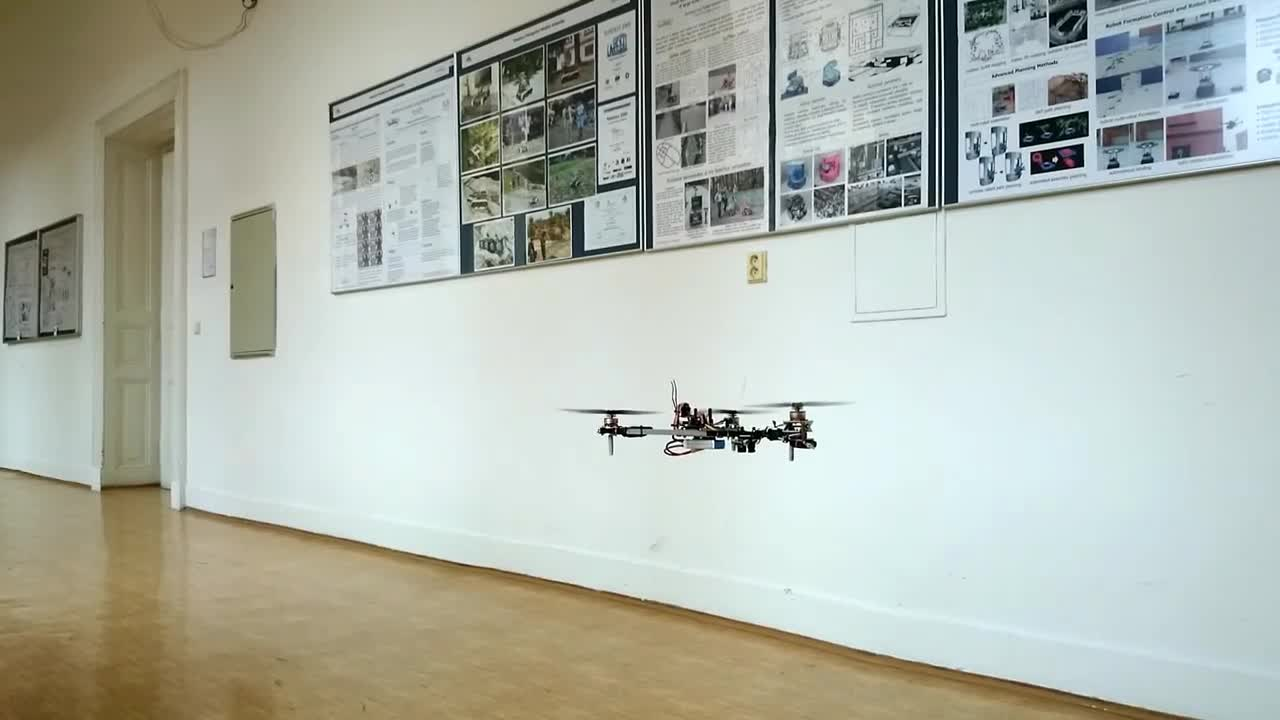
\includegraphics[width=0.8\textwidth]{fig/embedded_mpc_thumbnail.jpg}
        }{../videos/embedded_mpc.mp4}\\
        Video: \url{http://youtu.be/AXI_rkQRBaE}

      \end{center}
    \end{block}}

    \only<+>{\begin{block}{Embedded Model Predictive Control}
      \begin{center}
        \movie[autostart]{
          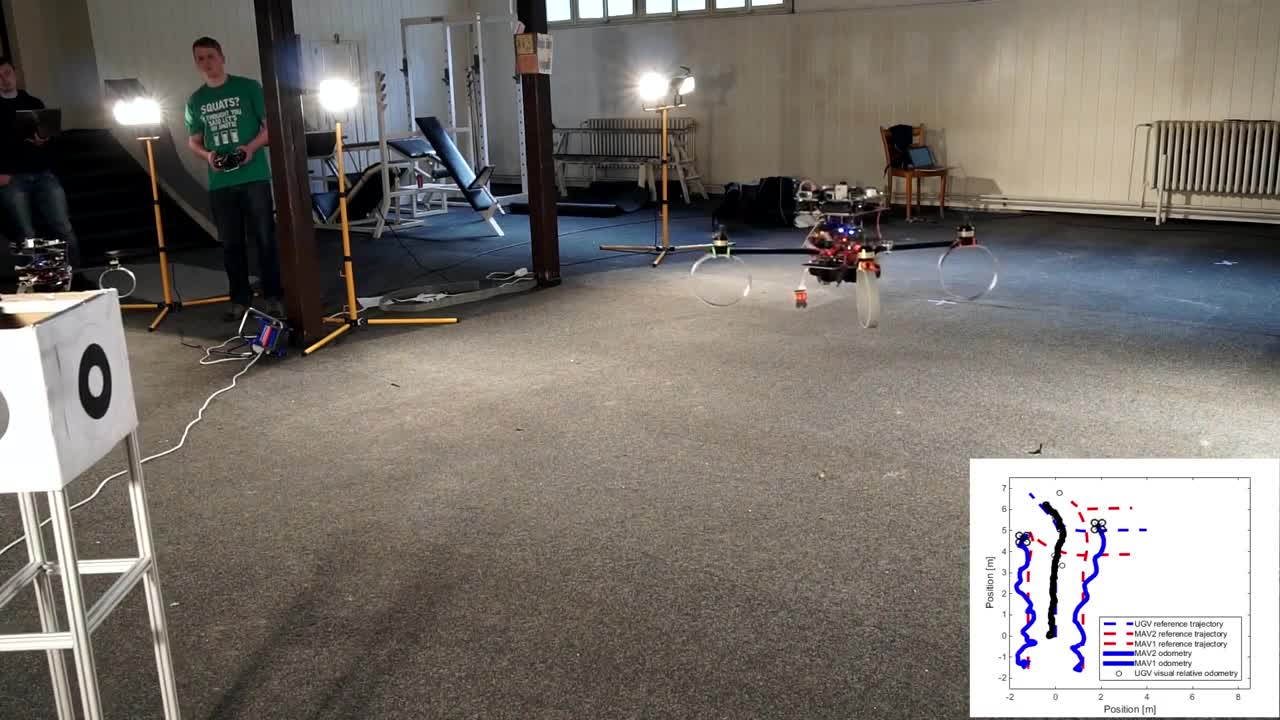
\includegraphics[width=0.8\textwidth]{fig/mmar_vojta_thumbnail.jpg}
        }{../videos/mmar_vojta.mp4}\\
        Video: \url{http://youtu.be/9Bpm4J31CgE}
      \end{center}
    \end{block}}

  \end{frame}

  \begin{frame}
    \frametitle{UAV Experimentation in MRS --- 2016--now}

    \begin{itemize}
      \onslide<1->{\item Custom and purpose-built hardware}
      \onslide<2->{\item Embedded software}
      \onslide<3->{\item Results: \cite{baca2016embedded}, \cite{spurny2016complex}, \cite{saska2016auro}, \cite{chudoba2016exploration}}
      \onslide<4->{\item {\color{red} Not Scalable! Bottlenecks everywhere: Embedded programming \emph{cumbersome}, simulating is difficult, system is hard-to-maintain, connecting sensors and peripheries is limited...}}
    \end{itemize}

  \end{frame}

  %%}

  %%{ Nowadays
  \begin{frame}
    \frametitle{Nowadays -- the system structure}

    \begin{block}{A typical pipeline structure revolves around a Linux computer.}
      \begin{figure}
        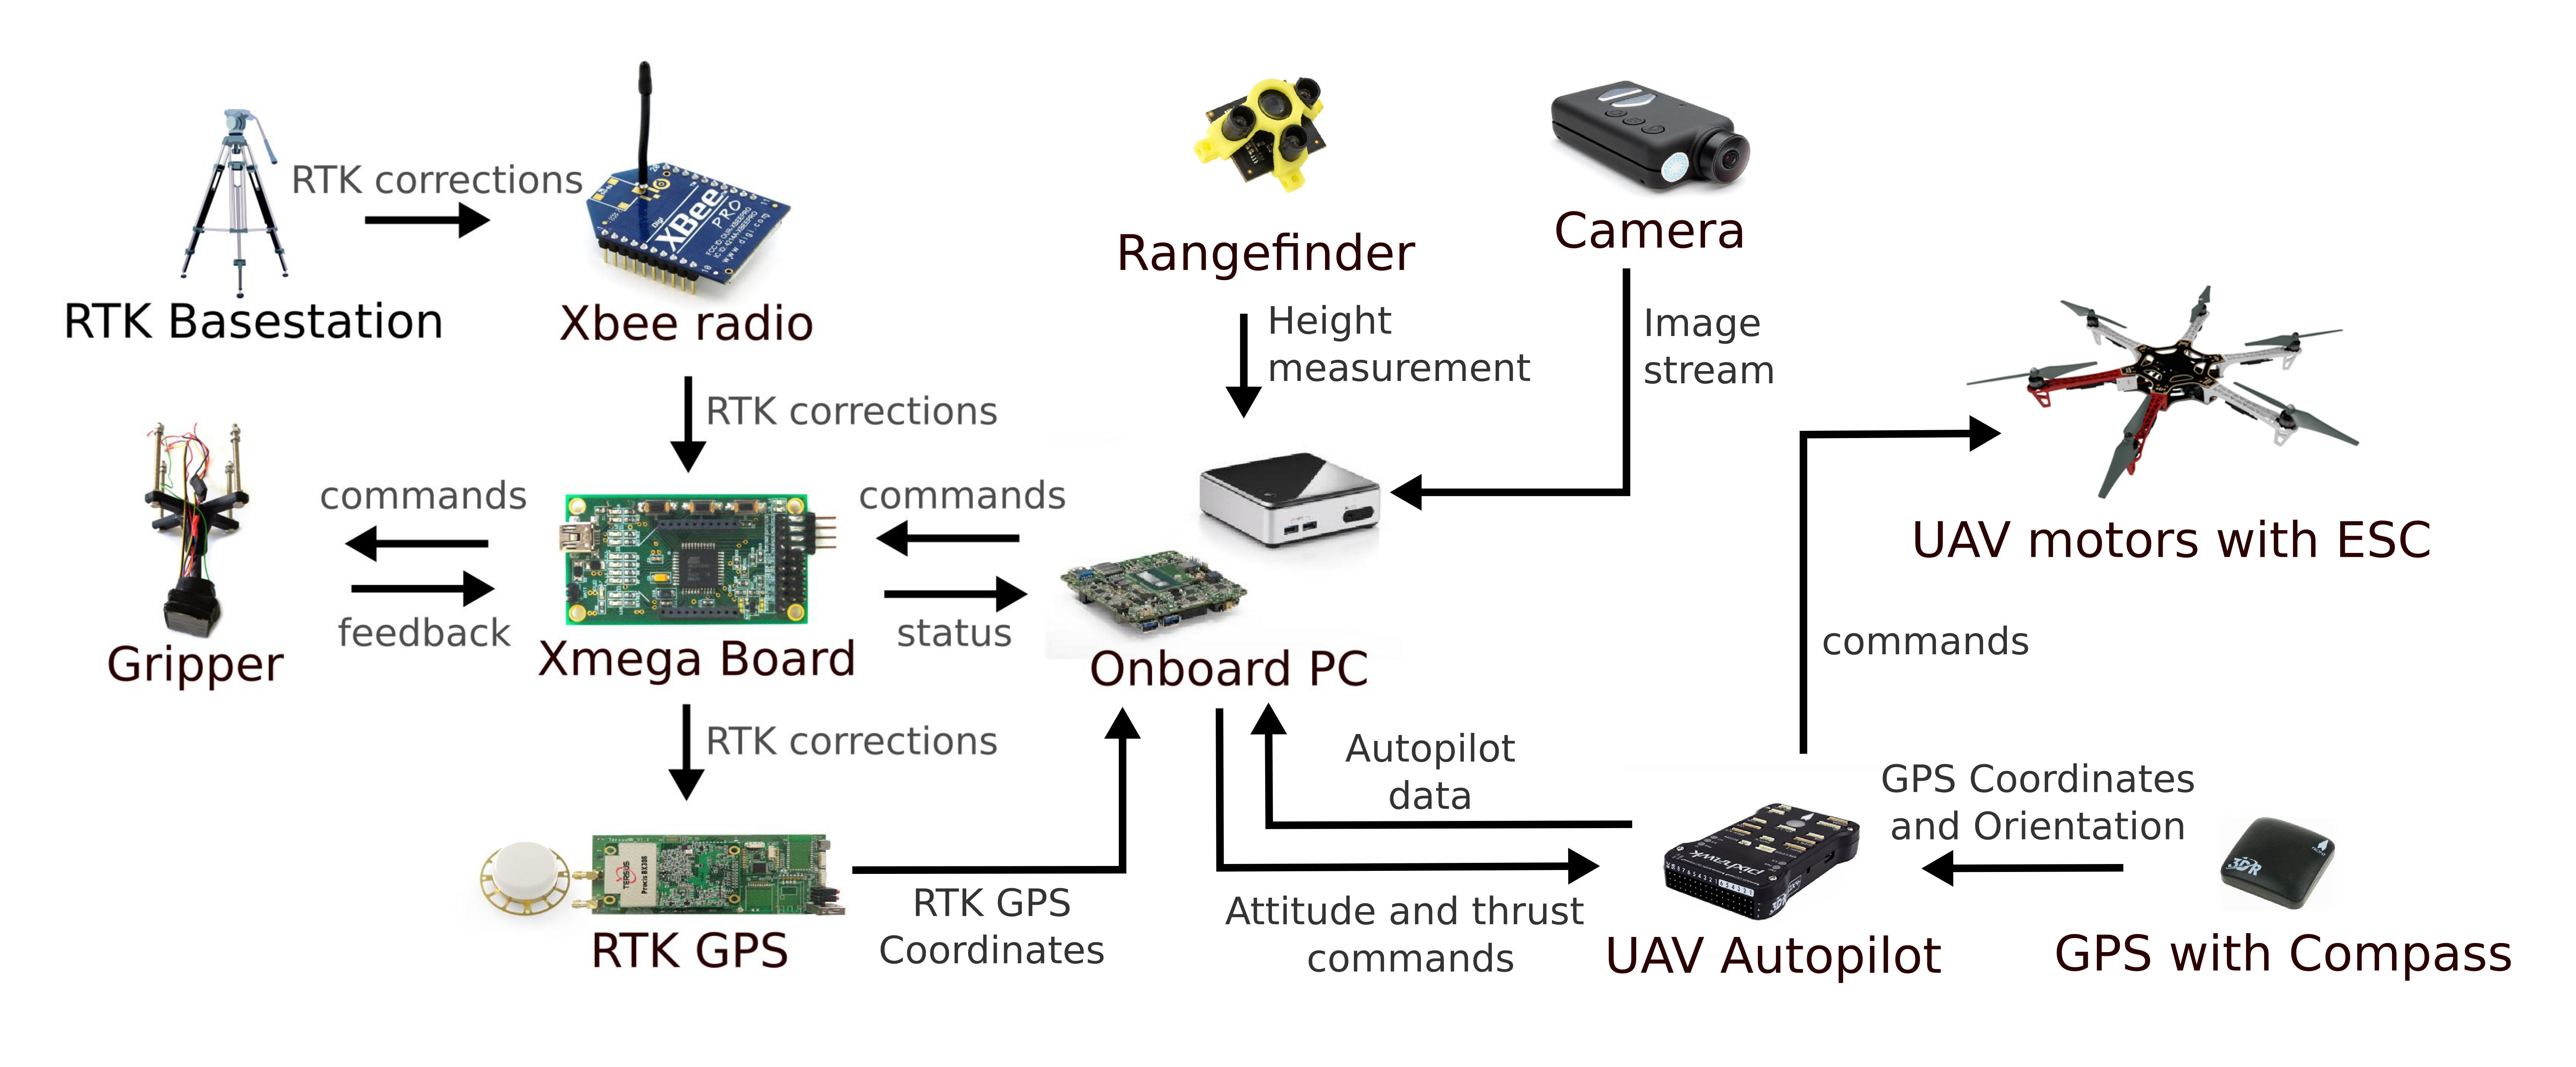
\includegraphics[width=1.0\textwidth]{fig/components.png}
      \end{figure}
    \end{block}

  \end{frame}
  %%}

  %%{ ROS -- Robot Operating System

  \begin{frame}
    \frametitle{ROS -- Robot Operating System}

    \begin{itemize}
      \item Middleware allowing communication between programs
      \item Integrates with \texttt{C++}, Python, Bash and Zshell
      \item Makes the transition from \emph{Matlab} to reality bearable
      \item Supported by sensor manufacturers
      \item Integration through the Linux terminal
      \item Handles the difficult stuff that nobody wants to program: time and clock management, logging, recording onboard data, visualization and plotting, parameter loading, static and dynamic transformations, etc.
      \item integrates to robotic simulators: Gazebo, Coppelia (V-REP)
    \end{itemize}

    \begin{figure}
      
\includegraphics[width=0.3\textwidth]{fig/ros_logo.jpg}
    \end{figure}

  \end{frame}

  %%}

  %% | ------------ Control pipeline - implementation ----------- |

  \section{UAV Control pipeline}
  \subsection{Control -- math point of view}

  %%{ UAV control pipepline
  \begin{frame}
    \frametitle{Control theory point of view}

    \begin{figure}
      \begin{adjustbox}{max totalsize={1.0\textwidth}{.85\textheight}, center}
        \pgfdeclarelayer{foreground}
\pgfsetlayers{background,main,foreground}

\tikzset{radiation/.style={{decorate,decoration={expanding waves,angle=90,segment length=4pt}}}}

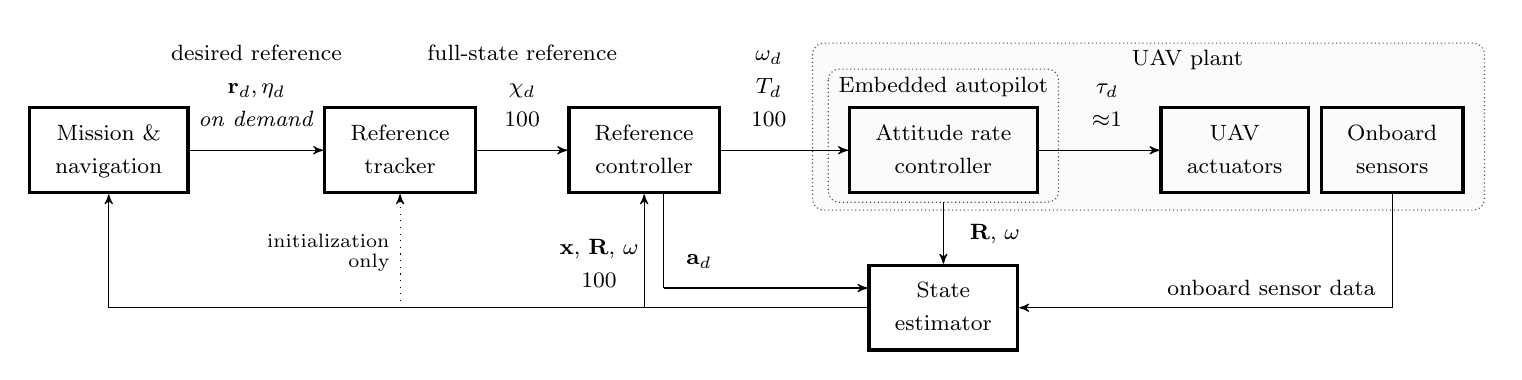
\begin{tikzpicture}[->,>=stealth', node distance=3.0cm,scale=1.0, every node/.style={scale=1.0}]

  %%{ nodes

  \node[state, shift = {(0.0, 0.0)}] (navigation) {
      \begin{tabular}{c}
        \footnotesize Mission \&\\
        \footnotesize navigation
      \end{tabular}
    };

  % \node[state, left of = navigation, shift = {(0.5, 0.0)}] (nimbro) {
  %     \begin{tabular}{c}
  %       \footnotesize Nimbro \\
  %       \footnotesize Network
  %     \end{tabular}
  %   };

  \node[state, right of = navigation, shift = {(0.7, 0)}] (tracker) {
      \begin{tabular}{c}
        \footnotesize Reference \\
        \footnotesize tracker
      \end{tabular}
    };

  \node[state, right of = tracker, shift = {(0.1, 0)}] (controller) {
      \begin{tabular}{c}
        \footnotesize Reference \\
        \footnotesize controller
      \end{tabular}
    };

  \node[state, right of = controller, shift = {(0.8, -0)}] (attitude) {
      \begin{tabular}{c}
        \footnotesize Attitude rate\\
        \footnotesize controller
      \end{tabular}
    };

  \node[state, right of = attitude, shift = {(0.7, -0)}] (actuators) {
      \begin{tabular}{c}
        \footnotesize UAV \\
        \footnotesize actuators
      \end{tabular}
    };

  \node[state, right of = actuators, shift = {(-1.0, -0)}] (sensors) {
      \begin{tabular}{c}
        \footnotesize Onboard \\
        \footnotesize sensors
      \end{tabular}
    };

  \node[state, below of = attitude, shift = {(0, 1.0)}] (estimator) {
      \begin{tabular}{c}
        \footnotesize State \\
        \footnotesize estimator
      \end{tabular}
    };

  %%}

  %%{ paths

  \path[->] ($(navigation.east) + (0.0, 0)$) edge [] node[above, midway, shift = {(0.0, 0.05)}] {
      \begin{tabular}{c}
        \footnotesize desired reference\\
        \footnotesize $\mathbf{r}_d, \eta_d$\\
        \footnotesize \textit{on demand}
    \end{tabular}} ($(tracker.west) + (0.0, 0.00)$);

  % \path[->] ($(nimbro.east) + (0.0, 0)$) edge [] node[above, midway, shift = {(0.0, 0.05)}] {
  %     \begin{tabular}{c}
  %   \end{tabular}} ($(navigation.west) + (0.0, 0.00)$);

  \path[->] ($(tracker.east) + (0.0, 0)$) edge [] node[above, midway, shift = {(0.0, 0.05)}] {
      \begin{tabular}{c}
        \footnotesize full-state reference\\
        \footnotesize $\bm{\chi}_d$\\
        \footnotesize \SI{100}{\hertz}
    \end{tabular}} ($(controller.west) + (0.0, 0.00)$);

  \path[->] ($(tracker.south |- estimator.west) + (0.0, 0.0)$) edge [dotted] node[left, midway, shift = {(0.2, 0.00)}] {
      \begin{tabular}{r}
        \scriptsize initialization\\[-0.5em]
        \scriptsize only
    \end{tabular}} ($(tracker.south) + (0.0, 0.00)$);

  \path[->] ($(controller.east) + (0.0, 0)$) edge [] node[above, midway, shift = {(-0.2, 0.05)}] {
      \begin{tabular}{c}
        \footnotesize $\bm{\omega}_d$\\
        \footnotesize $T_d$ \\
        \footnotesize \SI{100}{\hertz}
    \end{tabular}} ($(attitude.west) + (0.0, 0.00)$);

  \draw[-] ($(controller.south)+(0.25,0)$) -- ($(controller.south |- estimator.west) + (0.25, 0.25)$) edge [->] node[above, near start, shift = {(-0.2, 0.05)}] {
      \begin{tabular}{c}
        \footnotesize $\mathbf{a}_d$
    \end{tabular}} ($(estimator.west) + (0, 0.25)$);

  \path[->] ($(attitude.east) + (0.0, 0)$) edge [] node[above, midway, shift = {(0.1, 0.05)}] {
      \begin{tabular}{c}
        \footnotesize $\bm{\tau}_d$ \\
        \footnotesize $\approx$\SI{1}{\kilo\hertz}
    \end{tabular}} ($(actuators.west) + (0.0, 0.00)$);

  \path[-] ($(estimator.west)+(0, 0)$) edge [] node[above, near start, shift = {(-1.0, 0.0)}] {
      \begin{tabular}{c}
        \footnotesize $\mathbf{x}$, $\mathbf{R}$, $\bm{\omega}$\\
        \footnotesize \SI{100}{\hertz}
    \end{tabular}} ($(navigation.south |- estimator.west)$) -- ($(navigation.south |- estimator.west)$) edge [->,] ($(navigation.south)+(0, 0)$);

  % \path[-] ($(estimator.west)+(0, 0)$) edge [] node[above, near start, shift = {(-1.0, 0.0)}] {
  %     \begin{tabular}{c}
  %   \end{tabular}} ($(nimbro.south |- estimator.west)$) -- ($(nimbro.south |- estimator.west)$) edge [->,] ($(nimbro.south)+(0, 0)$);

  \path[->] ($(controller.south |- estimator.west)+(0, 0)$) edge [] ($(controller.south)$);

  \path[->] ($(attitude.south) + (0.0, -0.1)$) edge [] node[right, midway, shift = {(0.0, 0.00)}] {
      \begin{tabular}{c}
        \footnotesize $\mathbf{R}$, $\bm{\omega}$
    \end{tabular}} ($(estimator.north) + (0.0, 0.00)$);

  \path[-] ($(sensors.south)+(0, 0)$) edge [] ($(sensors.south |- estimator.east)$) -- ($(sensors.south |- estimator.east)$) edge [->,] node[above, near start, shift = {(-0.35, -0.1)}] {
      \begin{tabular}{c}
        \footnotesize onboard sensor data
    \end{tabular}}($(estimator.east)$);

  %%}

    % \draw[-, radiation, decoration={angle=45}] ($(nimbro.west) + (0.0, -0.0)$) -- +(0:-0.5);

  %%{ backgrounds

  \begin{pgfonlayer}{background}
    \path (attitude.west |- attitude.north)+(-0.45,0.8) node (a) {};
    \path (sensors.south -| sensors.east)+(+0.25,-0.20) node (b) {};
    \path[fill=gray!3,rounded corners, draw=black!70, densely dotted]
      (a) rectangle (b);
  \end{pgfonlayer}
  \node [rectangle, above of=actuators, shift={(-0.6,0.55)}, node distance=1.7em] (autopilot) {\footnotesize UAV plant};

  \begin{pgfonlayer}{background}
    \path (attitude.west |- attitude.north)+(-0.25,0.47) node (a) {};
    \path (attitude.south -| attitude.east)+(+0.25,-0.10) node (b) {};
    \path[fill=gray!3,rounded corners, draw=black!70, densely dotted]
      (a) rectangle (b);
  \end{pgfonlayer}
  \node [rectangle, above of=attitude, shift={(0,0.2)}, node distance=1.7em] (autopilot) {\footnotesize Embedded autopilot};

  %%}

\end{tikzpicture}

      \end{adjustbox}
    \end{figure}

    \begin{block}{\cite{baca2020mrs}}
      The MRS UAV System: Pushing the Frontiers of Reproducible Research, Real-world Deployment, and Education with Autonomous Unmanned Aerial Vehicles, preprint arXiv:2008.08050, 2020
    \end{block}

  \end{frame}
  %%}

  \subsection{Control -- implementation point of view}

  %%{ From theory to practical experiments

  %%{ Linear Kalman filter

  \begin{frame}
    \frametitle{From theory to practical experiments}

    \begin{columns}[c]

      \onslide<1->{\column{0.48\textwidth} % Left column and width
      \begin{block}{Linear Kalman Filter $\approx$ 10 lines}
        \begin{adjustbox}{max totalsize={1.0\textwidth}{.85\textheight}, center}
          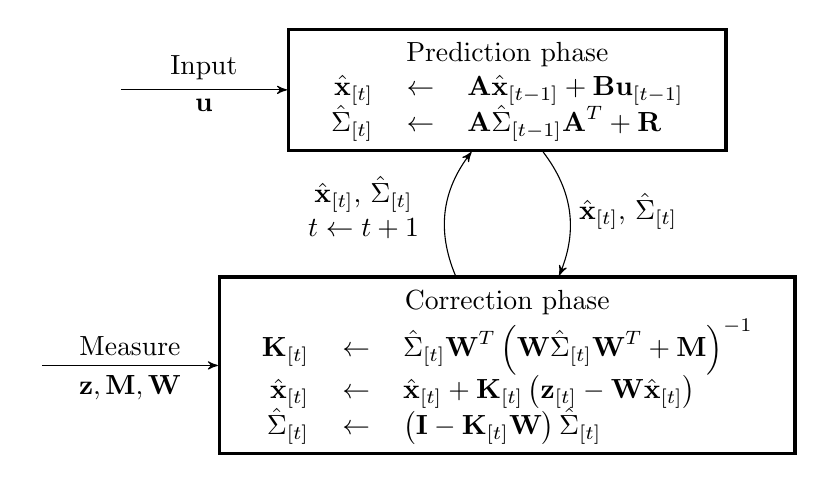
\begin{tikzpicture}[->,>=stealth']

% Position of PREDICTION
% Use previously defined 'state' as layout (see above)
% use tabular for content to get columns/rows
  % parbox to limit width of the listing
\node[state] (PREDICTION)
{
  \begin{tabular}{c}
  Prediction phase\\
    \begin{tabular}{rcl}
  $\hat{\textbf{x}}_{[t]}$ & $\leftarrow$ & $\textbf{A}\hat{\textbf{x}}_{[t-1]} + \textbf{B}\textbf{u}_{[t-1]}$ \\
    $\hat{\boldsymbol{\Sigma}}_{[t]}$ & $\leftarrow$ & $\textbf{A}\hat{\boldsymbol{\Sigma}}_{[t-1]}\textbf{A}^{T} + \textbf{R}$
    \end{tabular}
  \end{tabular}
};

  % State: CORRECTION with different content
\node[state,    	% layout (defined above)
  below of=PREDICTION, 	% Position is to the right of PREDICTION
  node distance=3.5cm, 	% distance to PREDICTION
  anchor=center] (CORRECTION) 	% posistion relative to the center of the 'box'
{%
  \begin{tabular}{c}
  Correction phase\\
    \begin{tabular}{rcl}
  $\textbf{K}_{[t]}$ & $\leftarrow$ & $\hat{\boldsymbol{\Sigma}}_{[t]}\textbf{W}^{T}\left(\textbf{W}\hat{\boldsymbol{\Sigma}}_{[t]}\textbf{W}^{T} + \textbf{M}\right)^{-1}$ \\
    $\hat{\textbf{x}}_{[t]}$ & $\leftarrow$ & $\hat{\textbf{x}}_{[t]} + \textbf{K}_{[t]}\left(\textbf{z}_{[t]} - \textbf{W}\hat{\textbf{x}}_{[t]}\right)$ \\
    $\hat{\boldsymbol{\Sigma}}_{[t]}$ & $\leftarrow$ & $\left(\mathbf{I} - \textbf{K}_{[t]}\textbf{W}\right)\hat{\boldsymbol{\Sigma}}_{[t]}$ \\
    \end{tabular}
  \end{tabular}
};

\node[nothing,    	% layout (defined above)
  left of=PREDICTION, 	% Position is to the right of QUERY
  node distance=5cm, 	% distance to QUERY
  anchor=center] (PRED_IN) 	% posistion relative to the center of the 'box'
{};

\node[nothing,    	% layout (defined above)
  left of=CORRECTION, 	% Position is to the right of QUERY
  node distance=6cm, 	% distance to QUERY
  anchor=center] (CORR_IN) 	% posistion relative to the center of the 'box'
{};

% draw the paths and and print some Text below/above the graph
\path (PREDICTION) 	edge[bend left=30]  node[anchor=west]
{
  $\hat{\textbf{x}}_{[t]}$, $\hat{\boldsymbol{\Sigma}}_{[t]}$
} (CORRECTION)
(CORRECTION) 	edge[bend left=30]  node[anchor=east]
{
  \begin{tabular}{c}
  $\hat{\textbf{x}}_{[t]}$, $\hat{\boldsymbol{\Sigma}}_{[t]}$ \\
    $t \leftarrow t + 1$
    \end{tabular}
} (PREDICTION)

(PRED_IN) edge[] node[anchor=south] {Input} node[anchor=north] {\textbf{u}} (PREDICTION)

  (CORR_IN) edge[] node[anchor=south] {Measure} node[anchor=north] {$\textbf{z}, \textbf{M}, \textbf{W}$} (CORRECTION);

  \end{tikzpicture}

        \end{adjustbox}
      \end{block}}

      \onslide<2>{\column{0.48\textwidth} % Right column and width
      \begin{block}{Linear Kalman Filter in practice}
        \begin{itemize}
          \item $\ge$ 1000 lines of \texttt{C++} code
          \item Real-world fusion \& estimation\\
            $\ge$ 10 000 lines of \texttt{C++} code
        \end{itemize}
      \end{block}}

    \end{columns}

  \end{frame}

  %%}

  %%{ Control

  \begin{frame}
    \frametitle{From theory to practical experiments}

    \begin{columns}[c]

      \column{0.48\textwidth} % Left column and width
      \onslide<1->{\vspace{-1em}
      \begin{block}{Geometric tracking controller $\approx$ 10 lines}
        \vspace{-1em}
        \tiny\begin{align}
          \mathbf{f}_d &= \minus m_e\mathbf{k}_p\circ \mathbf{e}_p \minusm_e\mathbf{k}_v\circ \mathbf{e}_v \plus m_e\ddot{\mathbf{r}}_d \minusm_eg\mathbf{\hat{e}}_3 \minus \mathbf{d}_w\circ \left[\begin{smallmatrix}
            1\\
            1\\
            0
          \end{smallmatrix}\right] \minus \mathbf{d}_b\circ \left[\begin{smallmatrix}
            1\\
            1\\
            0
          \end{smallmatrix}\right],\nonumber\\
          \mathbf{e}_R &= \frac{1}{2}\left(\mathbf{R}_d^\intercal\mathbf{R} - \mathbf{R}^\intercal\mathbf{R}_d\right),\nonumber\\
          \bm{\omega}_d &= \minus \mathbf{k}_R\circ \mathbf{e}_R \plus \bm{\omega}_j \minus \bm{\omega}_c,\nonumber
        \end{align}
        \vspace{-1em}
      \end{block}}

      \onslide<2->{
        \vspace{-0.5em}
        \begin{block}{MPC controller $\approx$ 100 lines}
          \vspace{-1em}
          \scriptsize{
            \begin{align*}
              & \min_{\mathbf{u}_{[1:n]}} \label{eq:mpc_cost}\nonumber
              & \frac{1}{2}\sum_{i=1}^{n-1}\left(\mathbf{e}^\intercal_{[i]}\mathbf{Q}\mathbf{e}_{[i]}\right) + \mathbf{e}^\intercal_{[n]}\mathbf{S}\mathbf{e}_{[n]}
            \end{align*}\begin{align*}
              \text{s.t.}~ \mathbf{x}_{m[i]} &= \mathbf{A}_m\mathbf{x}_{m[i-1]} \plus \mathbf{B}_m\mathbf{u}_{[i]}, &\forall i &\in \{1, \hdots, n\}\nonumber\label{eq:mpc_model}\\
              \mathbf{x}_{m[i]} &\leq \mathbf{x}_{\mathrm{max}}, &\forall i &\in \{1, \hdots, n\}\label{eq:mpc_max}\nonumber\\
              \mathbf{x}_{m[i]} &\geq \minus\mathbf{x}_{\mathrm{max}}, &\forall i &\in \{1, \hdots, n\}\label{eq:mpc_min}\nonumber \\
              \mathbf{u}_{[i]} \minus \mathbf{u}_{[i\minus1]} &\leq \dot{\mathbf{u}}_{\mathrm{max}} \Delta t, &\forall i &\in \{2, \hdots, n\}\label{eq:mpc_slew_min}\nonumber\\
              \mathbf{u}_{[i]} \minus \mathbf{u}_{[i\minus1]} &\geq \minus\dot{\mathbf{u}}_{\mathrm{max}} \Delta t, &\forall i &\in \{2, \hdots, n\}\label{eq:mpc_slew_max}\nonumber
            \end{align*}
            }
            \vspace{-1em}
        \end{block}}

        \column{0.48\textwidth} % Right column and width

        \onslide<3>{\begin{block}{UAV Control in practice}
          \begin{itemize}
            \item $\ge$ 10 000 lines of \texttt{C++} code
          \end{itemize}
        \end{block}}

    \end{columns}

  \end{frame}

  %%}

  %%{ From theory to practical experiments
  \begin{frame}
    \frametitle{From theory to practical experiments}

    \begin{columns}[c]

      \column{0.70\textwidth} % Left column and width
      \begin{block}{What needs to be solved outside of Matlab's sandbox?}
        \begin{itemize}
          \item crashes are expensive, so don't crash
          \item control references might not be feasible
          \item sensors can get disconnected during the flight
          \item takeoff and landing: \textbf{the most tricky part of the flight}
          \item mass (thus the model) can change during the flight
          \item controllers can be poorly tuned... handle instabilities
          \item acceleration and speed depend on the available sensors
          \item people are fallible, don't let them crash the drones
          \item not all states of UAV are allowed, even though controllers can reach them (upside down)
        \end{itemize}
      \end{block}

      \column{0.28\textwidth} % Right column and width
      \begin{block}{The failsafe core}
        \texttt{if (goingToCrash())}\\
        \texttt{~~~~dont();}
      \end{block}

    \end{columns}

  \end{frame}
  %%}

  %%}

  %% | --------------------- MRS UAV system --------------------- |

  \subsection{The MRS UAV System}

  %%{ The MRS UAV System
  \begin{frame}
    \frametitle{The MRS UAV System}

    \begin{itemize}
      \item Open-Source system for multirotor UAVs
      \item complete onboard execution
      \item outdoor/indoor/lab/real-world environment
      \item emphasis on safety and autonomy during experiments
      \item painless experiments from takeoff to landing
      \item extensible and powerful simulation
      \item relies on the PixHawk embedded flight controller
      \item safe for development and testing of new controllers
    \end{itemize}

  \end{frame}
  %%}

  %%{ Control pipeline implementation

  \begin{frame}
    \centering
    \begin{figure}

      \frametitle{Control -- implementation point of view}

      \begin{adjustbox}{max totalsize={1.0\textwidth}{.90\textheight}, center}
        \pgfdeclarelayer{foreground}
\pgfsetlayers{background,main,foreground}

\tikzset{radiation/.style={{decorate,decoration={expanding waves,angle=90,segment length=0.1em}}}}

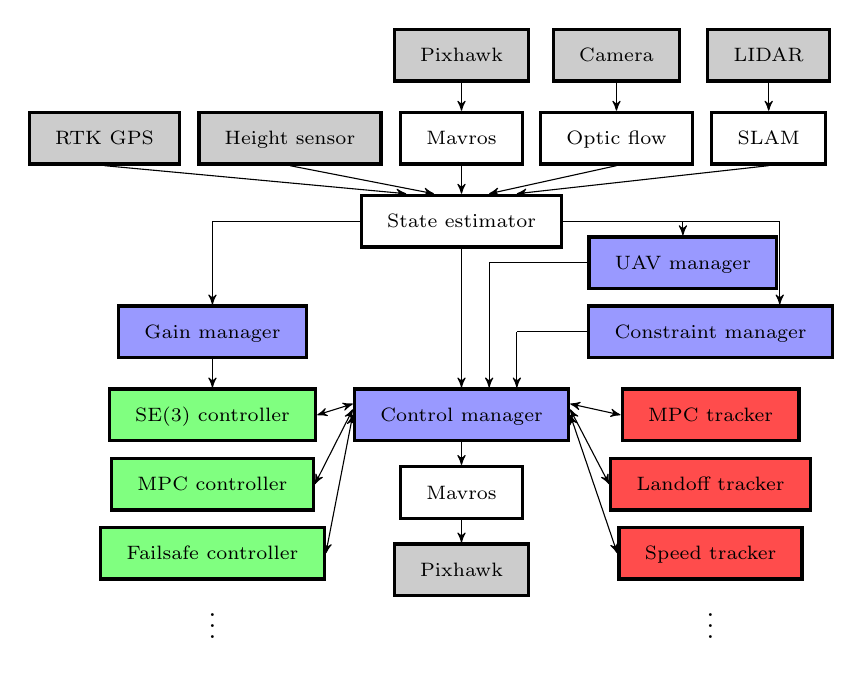
\begin{tikzpicture}[->,>=stealth', node distance=7.0em]

  %%{ nodes

  \node[state_blue, shift = {(0.0em, 0.0em)}] (control_manager) {
    \begin{tabular}{c}
      \scriptsize Control manager
    \end{tabular}
  };

  \node[state_red, right of = control_manager, shift = {(2.0em, 0.0em)}] (mpc_tracker) {
    \begin{tabular}{c}
      \scriptsize MPC tracker
    \end{tabular}
  };

  \node[state_red, below of = mpc_tracker, shift = {(0.0em, 4.5em)}] (landoff_tracker) {
    \begin{tabular}{c}
      \scriptsize Landoff tracker
    \end{tabular}
  };

  \node[state_blue, above of = mpc_tracker, shift = {(0.0em, -4.0em)}] (constraint_manager) {
    \begin{tabular}{c}
      \scriptsize Constraint manager
    \end{tabular}
  };

  \node[state_blue, above of = constraint_manager,  shift = {(-1.0em, -4.5em)}] (uav_manager) {
    \begin{tabular}{c}
      \scriptsize UAV manager
    \end{tabular}
  };

  \node[state_red, below of = landoff_tracker, shift = {(0.0em, 4.5em)}] (speed_tracker) {
    \begin{tabular}{c}
      \scriptsize Speed tracker
    \end{tabular}
  };

  \node[below of = speed_tracker, shift = {(0.0em, 4.5em)}] (dots_tracker) {
    \begin{tabular}{c}
      $\vdots$
    \end{tabular}
  };

  \node[state_green, left of = control_manager, shift = {(-2.0em, 0.0em)}] (se3_controller) {
    \begin{tabular}{c}
      \scriptsize SE(3) controller
    \end{tabular}
  };

  \node[state_green, below of = se3_controller, shift = {(0.0em, 4.5em)}] (mpc_controller) {
    \begin{tabular}{c}
      \scriptsize MPC controller
    \end{tabular}
  };

  \node[state_blue, above of = se3_controller, shift = {(0.0em, -4.0em)}] (gain_manager) {
    \begin{tabular}{c}
      \scriptsize Gain manager
    \end{tabular}
  };

  \node[state_green, below of = mpc_controller, shift = {(0.0em, 4.5em)}] (failsafe_controller) {
    \begin{tabular}{c}
      \scriptsize Failsafe controller
    \end{tabular}
  };

  \node[below of = failsafe_controller, shift = {(0.0em, 4.5em)}] (dots_controller) {
    \begin{tabular}{c}
      $\vdots$
    \end{tabular}
  };

  \node[state_white, below of = control_manager, shift = {(0.0em, 4.2em)}] (mavros2) {
    \begin{tabular}{c}
      \scriptsize Mavros
    \end{tabular}
  };

  % \node[state_white, above of = control_manager, shift = {(-2.2em, -3.0em)}] (nimbro) {
  %     \begin{tabular}{c}
  %       \scriptsize Nimbro
  %     \end{tabular}
  %   };

  \node[state_gray, below of = mavros2, shift = {(0.0em, 4.2em)}] (pixhawk2) {
    \begin{tabular}{c}
      \scriptsize Pixhawk
    \end{tabular}
  };

  \node[state_white, above of = control_manager, shift = {(0.0em, 0.0em)}] (estimator) {
    \begin{tabular}{c}
      \scriptsize State estimator
    \end{tabular}
  };

  \node[state_white, above of = estimator, shift = {(0.0em, -4.0em)}] (mavros) {
    \begin{tabular}{c}
      \scriptsize Mavros
    \end{tabular}
  };

  \node[state_gray, above of = mavros, shift = {(0.0em, -4.0em)}] (pixhawk) {
    \begin{tabular}{c}
      \scriptsize Pixhawk
    \end{tabular}
  };

  \node[state_white, right of = mavros, shift = {(-1.4em, 0.0em)}] (optic_flow) {
    \begin{tabular}{c}
      \scriptsize Optic flow
    \end{tabular}
  };

  \node[state_gray, above of = optic_flow, shift = {(0.0em, -4.0em)}] (camera) {
    \begin{tabular}{c}
      \scriptsize Camera
    \end{tabular}
  };

  \node[state_gray, left of = mavros, shift = {(0.8em, 0.0em)}] (height) {
    \begin{tabular}{c}
      \scriptsize Height sensor
    \end{tabular}
  };

  \node[state_gray, left of = height, shift = {(0.3em, 0.0em)}] (rtk) {
    \begin{tabular}{c}
      \scriptsize RTK GPS
    \end{tabular}
  };

  \node[state_white, right of = optic_flow, shift = {(-1.5em, 0.0em)}] (slam) {
    \begin{tabular}{c}
      \scriptsize SLAM
    \end{tabular}
  };

  \node[state_gray, above of = slam, shift = {(0.0em, -4.0em)}] (lidar) {
    \begin{tabular}{c}
      \scriptsize LIDAR
    \end{tabular}
  };

  %%}

  %%{ paths

  %% | ------------ connected sensor data to estimator ----------- |
  \path[-] ($(rtk.south)$) edge [->] ($(estimator.north) + (-2em, 0)$);
  \path[-] ($(height.south)$) edge [->] ($(estimator.north) + (-1.0em, 0)$);
  \path[-] ($(optic_flow.south)$) edge [->] ($(estimator.north) + (1.0em, 0)$);
  \path[-] ($(slam.south)$) edge [->] ($(estimator.north) + (2em, 0)$);
  \path[-] ($(mavros.south)$) edge [->] ($(estimator.north) + (0em, 0)$);

  \path[] ($(camera.south)$) edge [->] ($(optic_flow.north)$);

  %% | ---------------------- lidar to slam --------------------- |
  \path[-] ($(slam.north |- lidar.south)$) edge [->] ($(slam.north)$);

  %% | ----- connections from controllers to control manager ---- |
  \path ($(se3_controller.east)$) edge [<->] ($(control_manager.west) + (0, 0.4em)$);
  \path ($(mpc_controller.east)$) edge [<->] ($(control_manager.west) + (0, 0.20em)$);
  \path ($(failsafe_controller.east)$) edge [<->] ($(control_manager.west) + (0, 0.0em)$);
  % \path ($(failsafe_controller.east |- dots_controller.east)$) edge [<->] ($(control_manager.west) + (0, -0.2em)$);

  %% | ------ connections from trackers to control manager ------ |
  \path ($(speed_tracker.west)$) edge [<->] ($(control_manager.east) + (0, 0.00em)$);
  \path ($(landoff_tracker.west)$) edge [<->] ($(control_manager.east) + (0, 0.20em)$);
  \path ($(mpc_tracker.west)$) edge [<->] ($(control_manager.east) + (0, 0.40em)$);
  % \path ($(speed_tracker.west |- dots_tracker.west)$) edge [<->] ($(control_manager.east) + (0, -0.20em)$);

  %% | ------------------- gain manager to se3 ------------------ |
  \path[-] ($(gain_manager.south)$) edge [->] ($(se3_controller.north)$);

  %% | ---------- constraint manager to control manager --------- |
  \draw[-] ($(constraint_manager.west)$) -- ($(control_manager.north |- constraint_manager.west) + (2em, 0)$) edge [->] ($(control_manager.north) + (2em, 0)$);

  %% | ------------- control manager to uav manager ------------- |
  \draw[-] ($(uav_manager.west)$) -- ($(control_manager.north |- uav_manager.west) + (1em, 0)$) edge [->] ($(control_manager.north) + (1em, 0)$);

  %% | --------------- estimator to control manager -------------- |
  \path ($(estimator.south) + (0.0em, 0)$) edge [->] ($(control_manager.north) + (0.0em, 0)$);

  %% | --------------- estimator to uav manager -------------- |
  \draw[-] ($(estimator.east)$) -- ($(uav_manager.north |- estimator.east) + (0em, 0)$) edge [->] ($(uav_manager.north) + (0em, 0)$);

  %% | ---------------- estimator to gain manager --------------- |
  \draw[-] ($(estimator.west)$) -- ($(gain_manager.north |- estimator.west) + (0em, 0)$) edge [->] ($(gain_manager.north) + (0em, 0)$);

  %% | ------------- estimator to constraint manager ------------ |
  \draw[-] ($(estimator.east)$) -- ($(constraint_manager.north |- estimator.east) + (2.5em, 0)$) edge [->] ($(constraint_manager.north) + (2.5em, 0)$);

  %% | ------------------------- pixhawk ------------------------ |
  \path ($(pixhawk.south)$) edge [->] ($(mavros.north)$);

  %% | ------------------------ pixhawk 2 ----------------------- |
  \path ($(mavros2.north |- control_manager.south)$) edge [->] ($(mavros2.north)$);
  \path ($(pixhawk2.north)$) edge [<-] ($(mavros2.south)$);

  % %% | ------------------------- nimbro ------------------------- |
  % \path ($(nimbro.south)$) edge [->] ($(nimbro.south |- control_manager.north)$);

  %%}

  %%{ backgrounds

  % \begin{pgfonlayer}{background}
  %   \path (se3_controller.east |- se3_controller.north)+(+0.3, 0.3) node (a) {};
  %   \path (attitude_controller.south -| se3_controller.west)+(-0.3,-0.3) node (b) {};
  %   \path[fill=black!70, draw=black!50, dashed]
  %   (a) rectangle (b);
  %   \path (a) -- node [midway, shift = {(-5.5, -1.0)}] {\begin{tabular}{c}
  %       \scriptsize Controllers\\
  %       \scriptsize (ROS Plugins)
  %   \end{tabular}} (a);
  % \end{pgfonlayer}

  % \begin{pgfonlayer}{background}
  %   \path (landoff_tracker.east |- landoff_tracker.north)+(+0.3, 0.3) node (a) {};
  %   \path (csv_tracker.south -| landoff_tracker.west)+(-0.3,-0.3) node (b) {};
  %   \path[fill=black!70, draw=black!50, dashed]
  %   (a) rectangle (b);
  %   \path (a) -- node [midway, shift = {(1.5, -1.0)}] {\begin{tabular}{c}
  %       \scriptsize Trackers\\
  %       \scriptsize (ROS Plugins)
  %   \end{tabular}} (a);
  % \end{pgfonlayer}

  %%}

\end{tikzpicture}

      \end{adjustbox}

    \end{figure}

  \end{frame}

  %%}

  %%{ MRS UAV System --- Feedforward Trackers

  \begin{frame}
    \frametitle{MRS UAV System --- Feedforward Trackers}

    \begin{itemize}
      \item receive high-level references from a navigation software, those are generally
        a single \textbf{position} \& \textbf{heading} reference,
        a \textbf{trajectory}, consisting of several \textbf{position} \& \textbf{heading} references separated by a fixed time constant.
      \item generate all-state and feasible reference for the controllers, which consists of
        desired position, velocity, acceleration, heading, and heading rate
      \item trackers are provided with a set of state constraints that should be satisfied at all times.
      \item loaded as plugins to the \emph{ControlManager}
    \end{itemize}

    \begin{block}{Available trackers}
      MPC tracker, Landoff tracker, Joy tracker, Speed tracker, \hdots
    \end{block}

    \begin{block}{\cite{baca2020mrs}}
      \url{http://github.com/ctu-mrs/mrs_uav_trackers}
    \end{block}

  \end{frame}

  %%}

  %%{ MRS UAV System --- Feedback Controllers

  \begin{frame}
    \frametitle{MRS UAV System --- Feedback Controllers}

    \begin{itemize}
      \item receive a current UAV state estimate
      \item receive the all-state reference from reference trackers
      \item control the states of the UAV by outputting a desired angular rate (or desired orientation) and desired collective thrust
      \item loaded as plugins to the \emph{ControlManager}
    \end{itemize}

    \begin{block}{Available controllers}
      SE(3) controller, MPC controller, Emergency controller, Failsafe controller
    \end{block}

    \begin{block}{\cite{baca2020mrs}}
      \url{http://github.com/ctu-mrs/mrs_uav_controllers}
    \end{block}

  \end{frame}

  %%}

  %%{ MRS UAV System --- Control Manager

  \begin{frame}
    \frametitle{MRS UAV System --- Control Manager}

    \onslide<+>{\begin{itemize}
      \item integrates the control and tracking part of the MRS UAV pipeline
      \item dynamically loads \textbf{controllers} and \textbf{trackers} plugins
      \item subscribes to the UAV state estimate and provides it to all loaded trackers and controllers
      \item outputs the attitude rate command the Pixhawk flight controller
      \item provides constraints for trackers through a common interface
      \item allows in-mid-air switching of feedback controllers and reference trackers
      \item provides an interface between to UAV and a user
      \item \textbf{provides safety features}
    \end{itemize}}

    \onslide<+>{
      \begin{block}{Safety features}
        \begin{itemize}
          \item emergency hover
          \item emergency landing
          \item feedforward failsafe landing
        \end{itemize}
      \end{block}
    }

    \begin{block}<1-2>{\cite{baca2020mrs}}
      \url{http://github.com/ctu-mrs/mrs_uav_managers}
    \end{block}

  \end{frame}

  %%}

  %%{ MRS UAV System --- UAV Manager

  \begin{frame}
    \frametitle{MRS UAV System --- UAV Manager}


    \begin{block}{\cite{baca2020mrs}}
      \url{http://github.com/ctu-mrs/mrs_uav_managers}
    \end{block}

  \end{frame}

  %%}

  %%{ MRS UAV System --- Odometry

  \begin{frame}
    \frametitle{MRS UAV System --- Odometry}


    \begin{block}{\cite{baca2020mrs}}
      \url{http://github.com/ctu-mrs/mrs_uav_odometry}
    \end{block}

  \end{frame}

  %%}

  %%{ MRS UAV System --- Simulation

  \begin{frame}
    \frametitle{MRS UAV System --- Simulation}

    \begin{block}{\cite{baca2020mrs}}
      \url{http://github.com/ctu-mrs/mrs_simulation}
    \end{block}

  \end{frame}

  %%}

  %%{ MRS UAV System --- Example Packages

  \begin{frame}
    \frametitle{MRS UAV System --- Example ROS Packages}

    \begin{block}{\cite{baca2020mrs}}
      \url{http://github.com/ctu-mrs/example_ros_packages}
    \end{block}

  \end{frame}

  %%}

  %%{ Preprint paper
  \begin{frame}
    \frametitle{Preprint}

    \begin{block}{The MRS UAV System paper preprint --- arXiv:2008.0805}
      \begin{figure}
        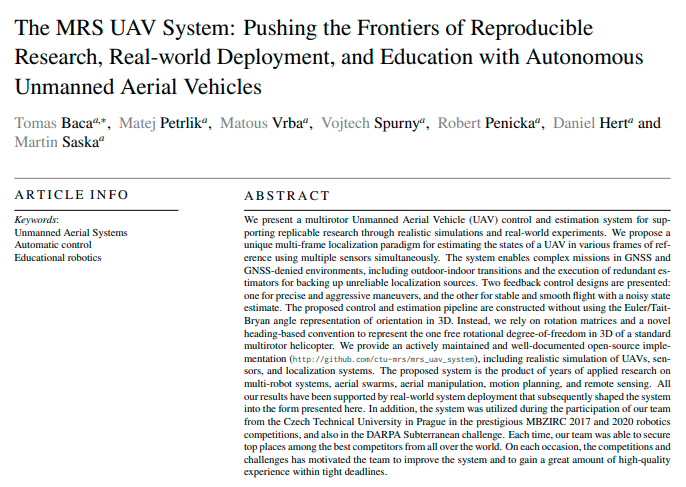
\includegraphics[width=0.7\textwidth]{fig/mrs_uav_system_paper.png}
      \end{figure}
    \end{block}

  \end{frame}
  %%}

  %% --------------------------------------------------------------
  %% |                      Linux environment                     |
  %% --------------------------------------------------------------

  \section{Software tools at our disposal}
  \subsection{terminal, shell, Tmux, Vim, ROS}

  %%{ Linux terminal & shell

  \begin{frame}
    \frametitle{Linux terminal \& shell}

    \begin{block}{A Linux terminal}
      \begin{figure}
        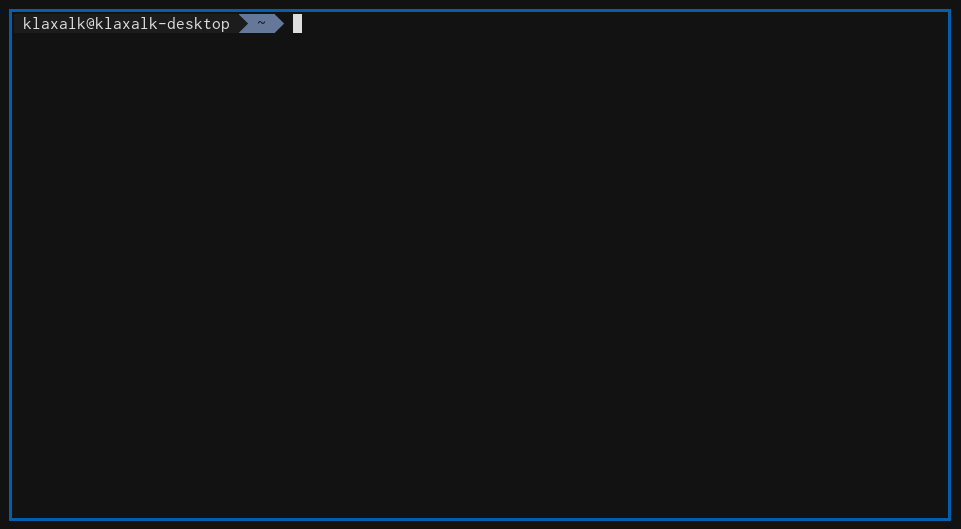
\includegraphics[width=0.9\textwidth]{fig/terminal.png}
      \end{figure}
    \end{block}

  \end{frame}

  %%}

  %%{ Tmux & Terminal multiplexer

  \begin{frame}

    \frametitle{Tmux -- Terminal multiplexer}

    \begin{block}{Tmux in the Linux terminal}
      \begin{figure}
        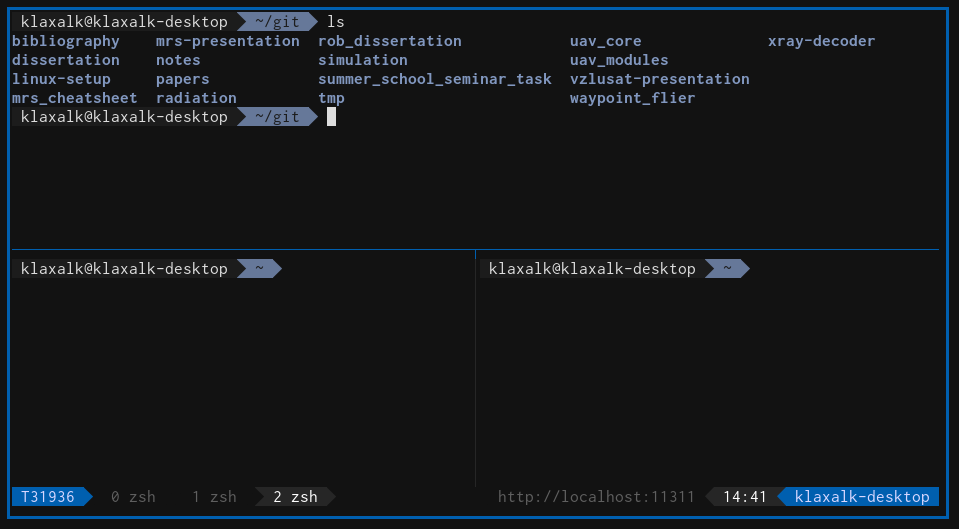
\includegraphics[width=0.9\textwidth]{fig/tmux.png}
      \end{figure}
    \end{block}

  \end{frame}

  %%}

  %%{ Ranger

  \begin{frame}

    \frametitle{Ranger -- terminal file manager}

    \begin{block}{Ranger}
      \begin{figure}
        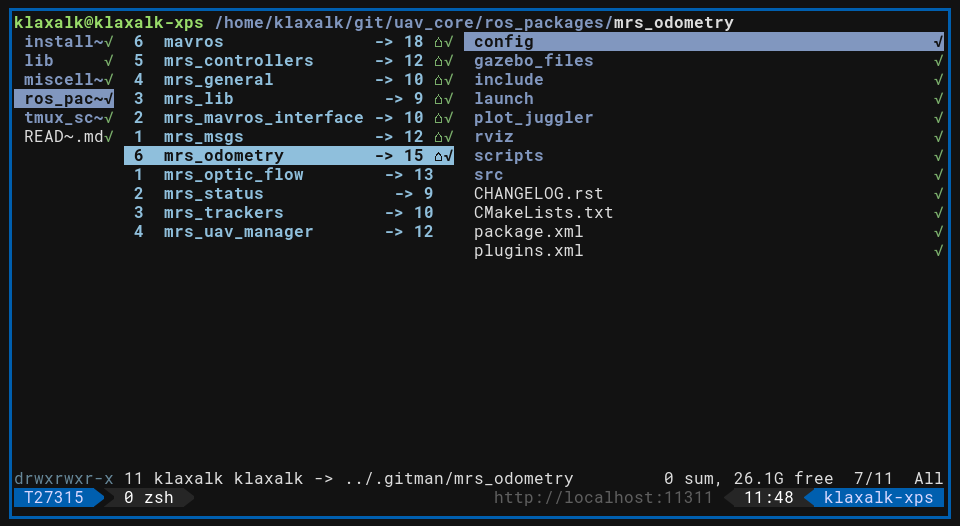
\includegraphics[width=0.9\textwidth]{fig/ranger.png}
      \end{figure}
    \end{block}

  \end{frame}

  %%}

  %%{ Vim -- modal, modular, modern

  \begin{frame}
    \frametitle{Vim -- modal, modular, modern}

    \begin{block}{Vim in (Tmux in (Linux Terminal)}
      \begin{figure}
        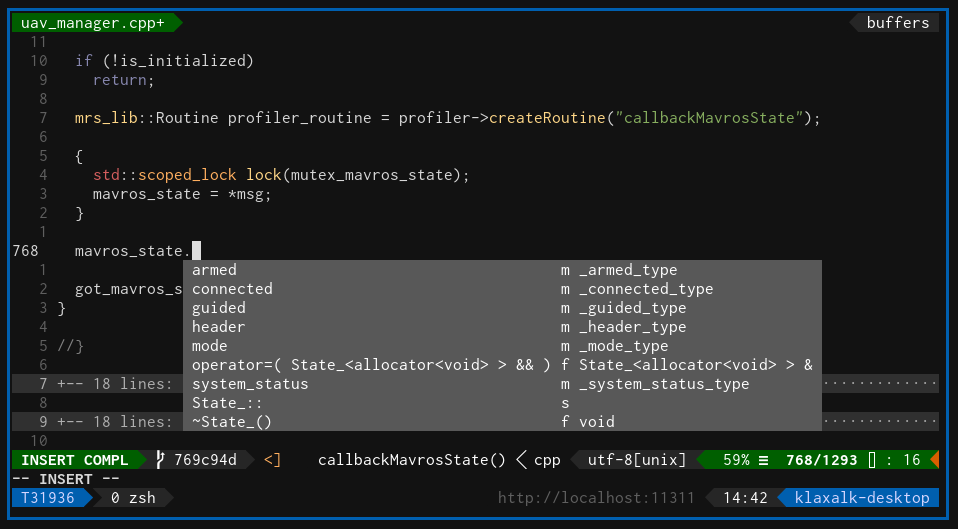
\includegraphics[width=0.9\textwidth]{fig/vim.png}
      \end{figure}
    \end{block}

  \end{frame}

  %%}

  %%{ Vim -- modal, modular, modern

  \begin{frame}
    \frametitle{Vim -- modal, modular, modern}

    \begin{block}{Terminal in (Vim in (Tmux in (Linux Terminal))}
      \begin{figure}
        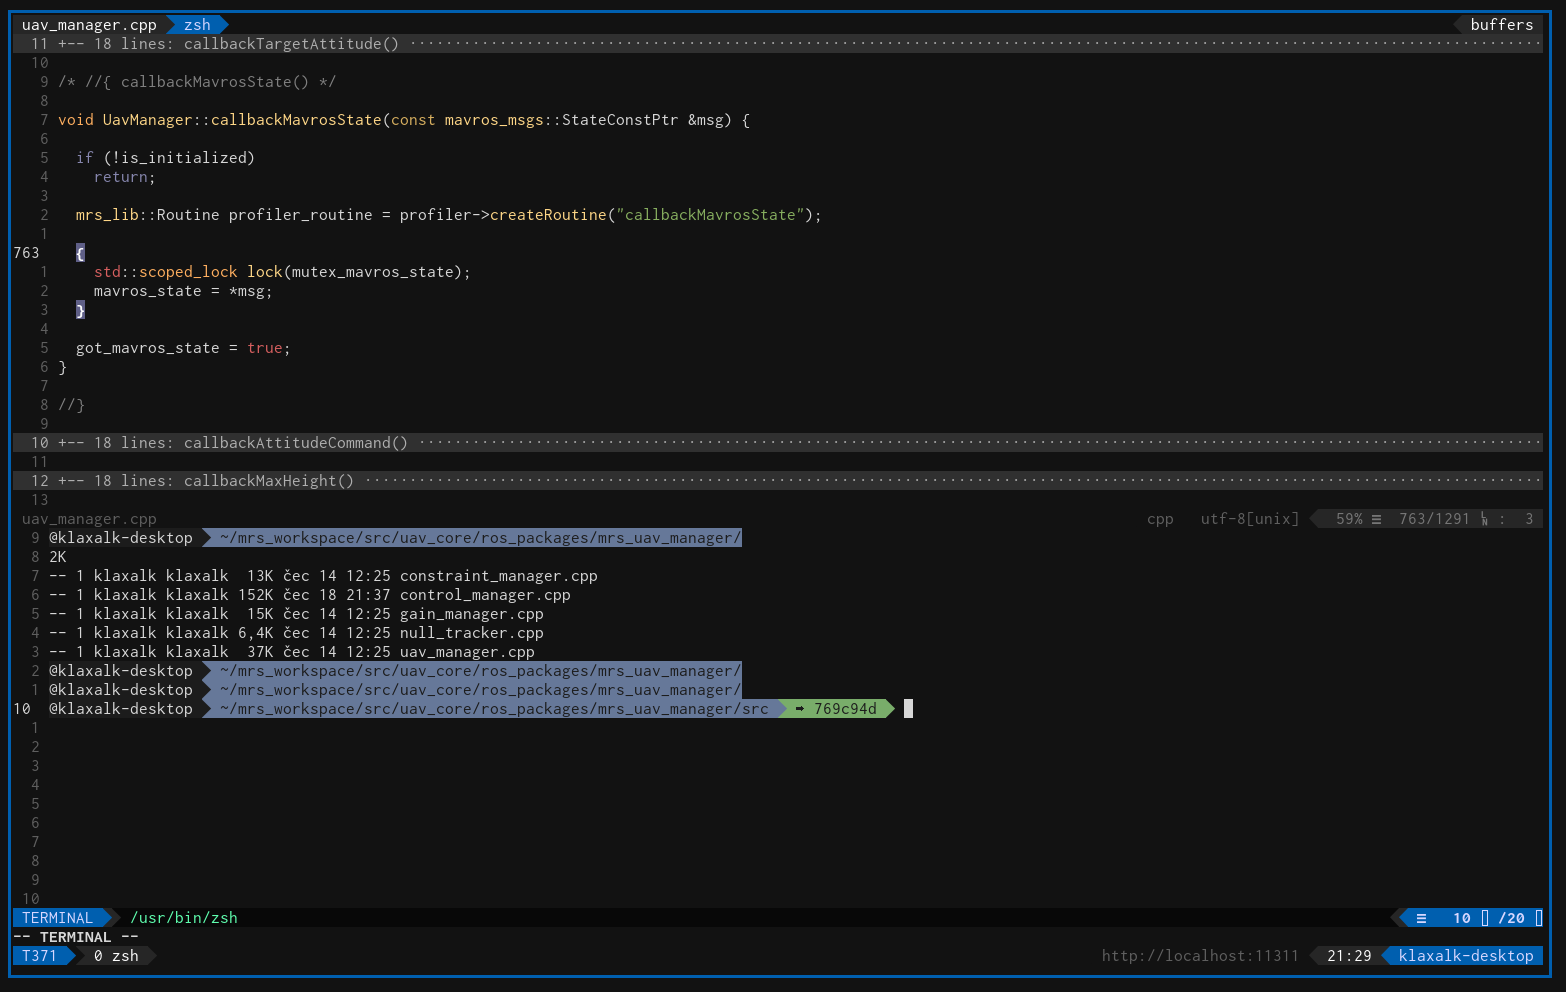
\includegraphics[width=0.8\textwidth]{fig/terminal_in_vim.png}
      \end{figure}
    \end{block}

  \end{frame}

  %%}

  %% | ---------------------- The simulator --------------------- |

  \section{MRS simulation stack}

  \subsection{Gazebo/ROS, spawn}

  %%{ Gazebo/ROS simulator
  \begin{frame}
    \frametitle{Gazebo/ROS simulator}

    \begin{figure}
      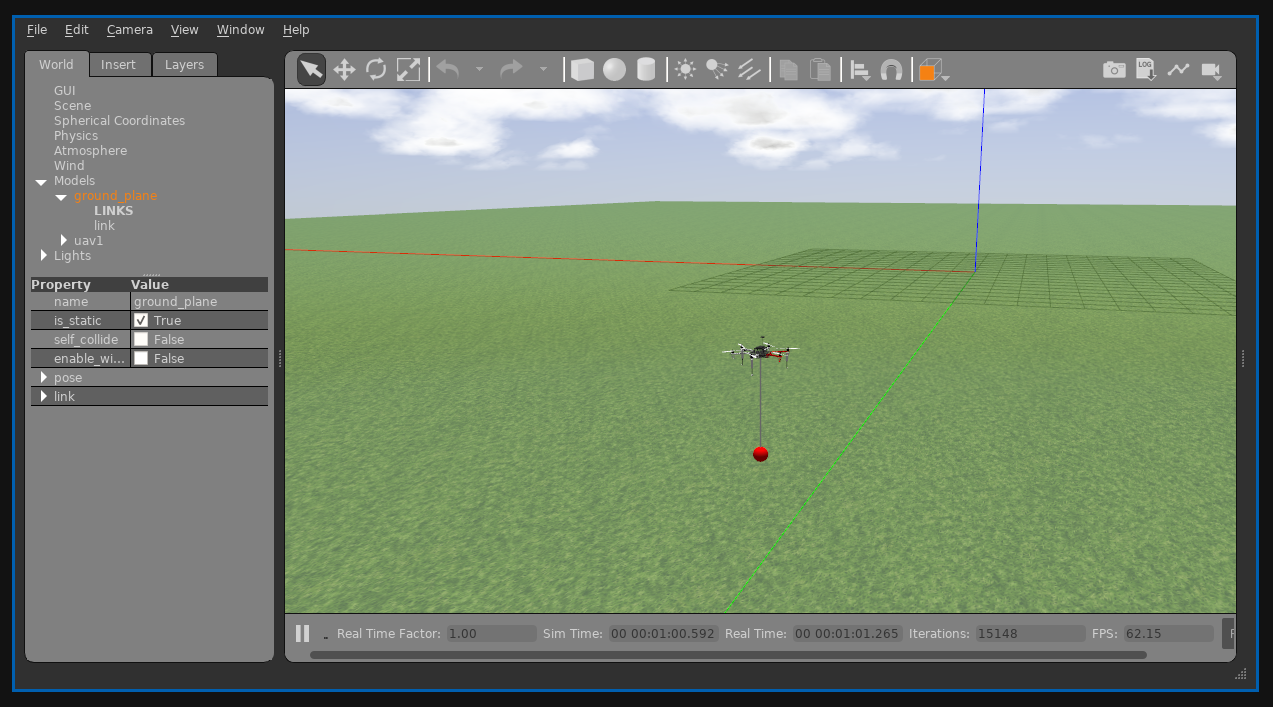
\includegraphics[width=1.0\textwidth]{fig/gazebo.png}
    \end{figure}

  \end{frame}
  %%}

  %%{ Spawning drones to the simulator
  \begin{frame}
    \frametitle{Spawning drones to the simulator}

    \begin{figure}
      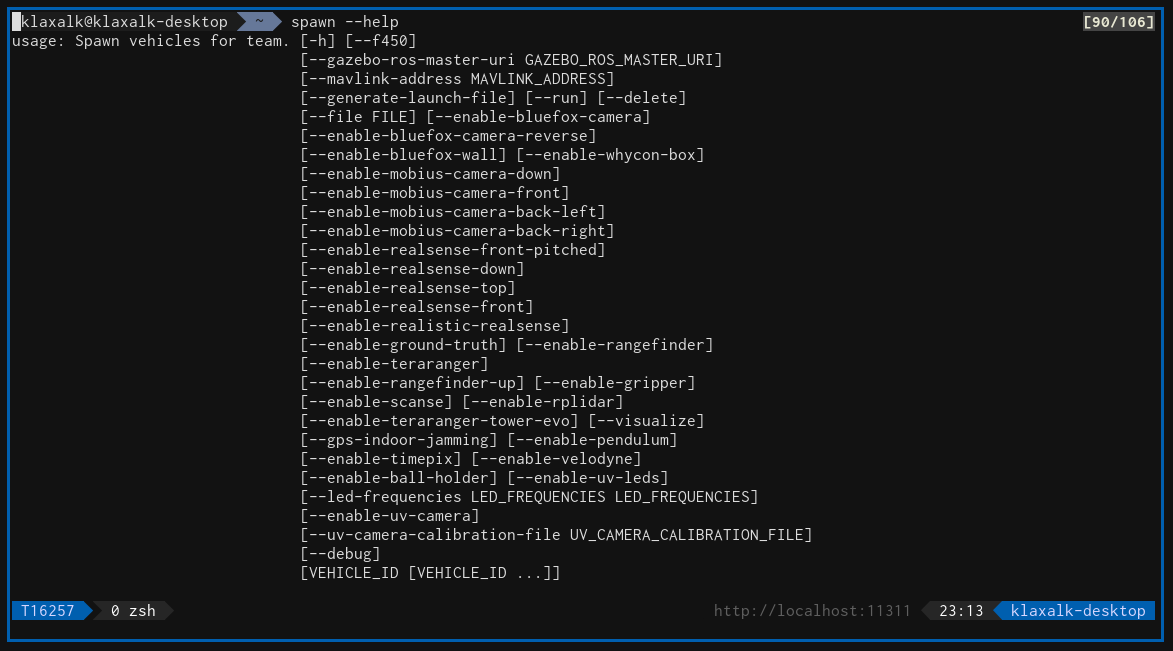
\includegraphics[width=1.0\textwidth]{fig/spawn.png}
    \end{figure}

  \end{frame}
  %%}

  %%{ Show the live demo
  \begin{frame}
    \frametitle{Show the live demo}

    \begin{center}
      \large Now is the time to show the Live demo.\\
      \vspace{2em}
      1st law of robotics: never give a robotic demo!
    \end{center}

  \end{frame}
  %%}

  %% | ------------------- Seminar assignments ------------------ |

  \section{Summer School seminar}
  \subsection{the MTSPN problem}
  \subsection{running the planner, w/ and w/o ROS}

  %%{ Seminars' assignemnt -- MTSPN

  \begin{frame}
    \frametitle{Seminars' assignment -- MTSPN}

    \begin{columns}[c]

      \column{0.48\textwidth} % Left column and width
      \begin{block}{A sample map of points}
        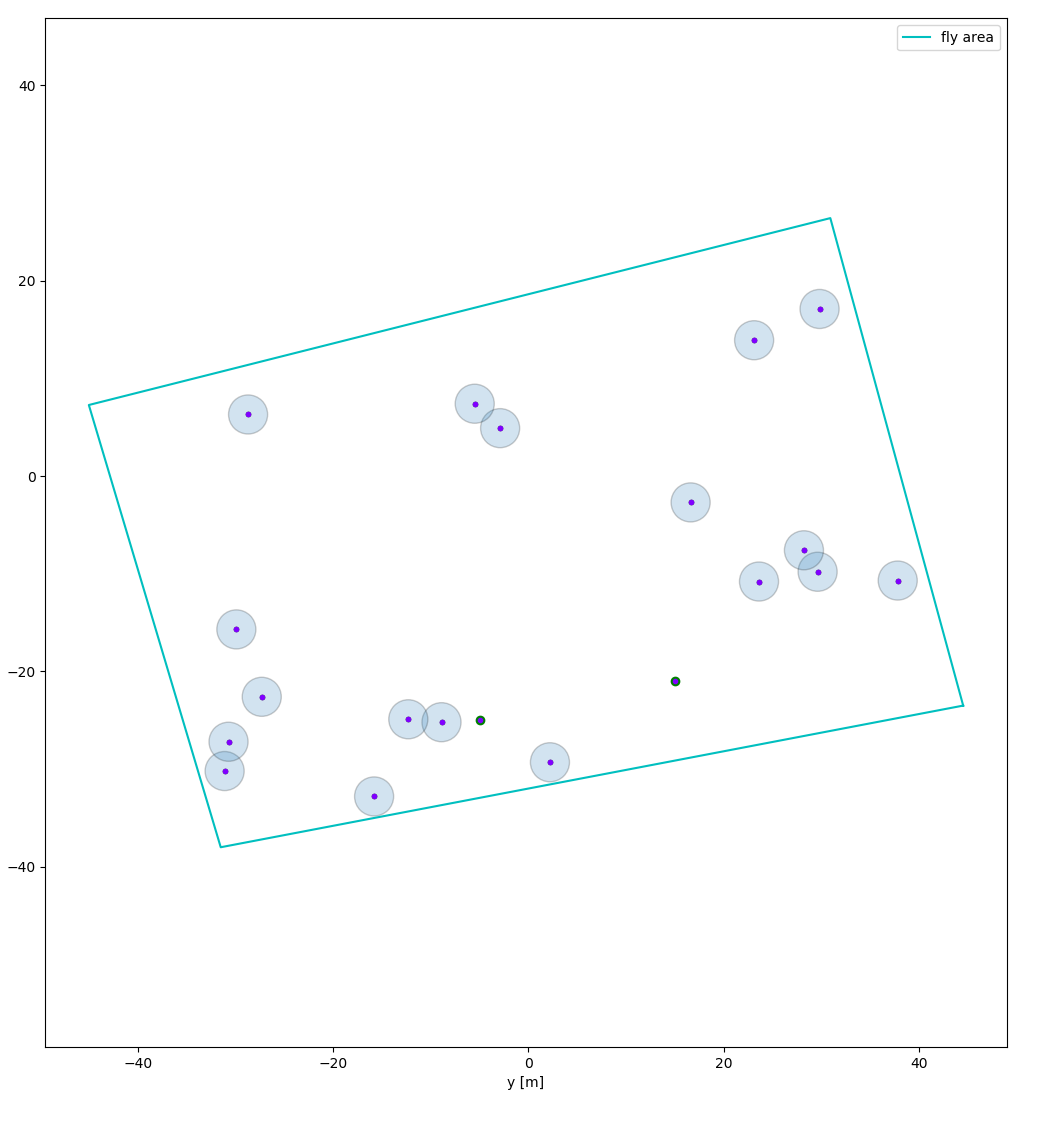
\includegraphics[width=1.0\textwidth]{fig/tsp_points.png}
      \end{block}

      \column{0.48\textwidth} % Right column and width
      \begin{block}{Multiple (Dubins) Traveling Salesman Problems (with Neighborhoods)}
        \begin{itemize}
          \item \unit{2}{m} neighborhood around each point
          \item each point's neighborhood has to be visited by any of the drones
          \item drones' min mutual distance: \unit{5}{m}
          \item faster total time wins
        \end{itemize}
      \end{block}

      \begin{block}{UAV's constraints}
        \begin{itemize}
          \item trajectory sampled at \unit{5}{Hz}
          \item max. speed \unit{7}{m/s}
          \item max. acceleration \unit{2.5}{m/s^2}
          \item UAV's start = finish
        \end{itemize}
      \end{block}

    \end{columns}

  \end{frame}

  %%}

  %%{ An example solution
  \begin{frame}
    \frametitle{An example solution of MTSP}

    \begin{figure}
      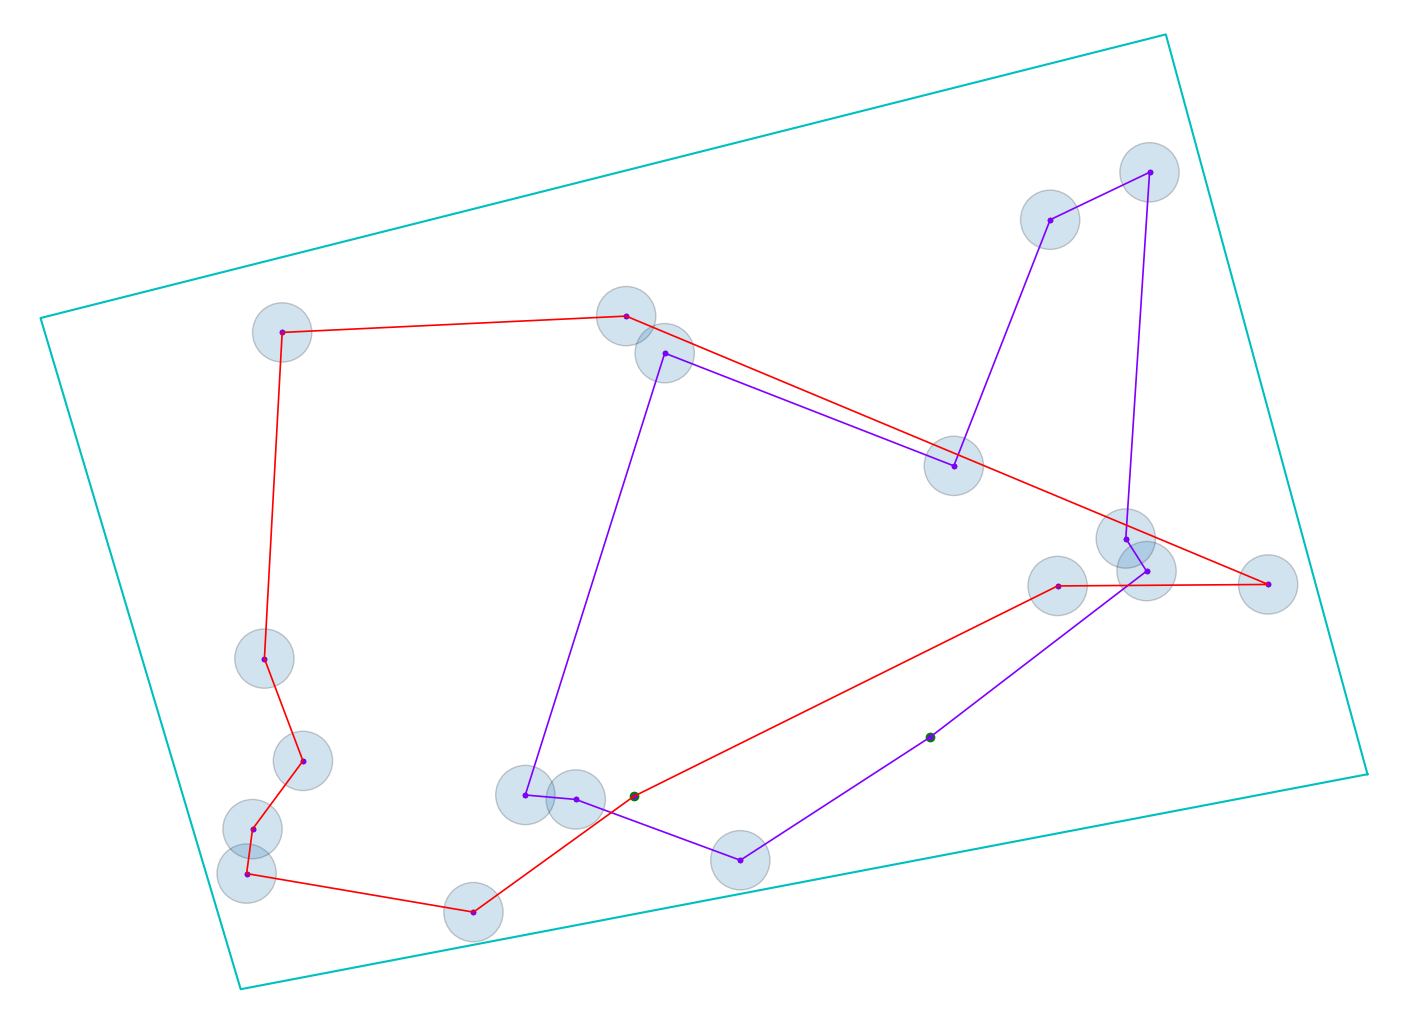
\includegraphics[width=0.8\textwidth]{fig/tsp_segments_center.png}
    \end{figure}

  \end{frame}
  %%}

  %%{ With neighborhoods
  \begin{frame}
    \frametitle{An example solution with neighborhoods}

    \begin{figure}
      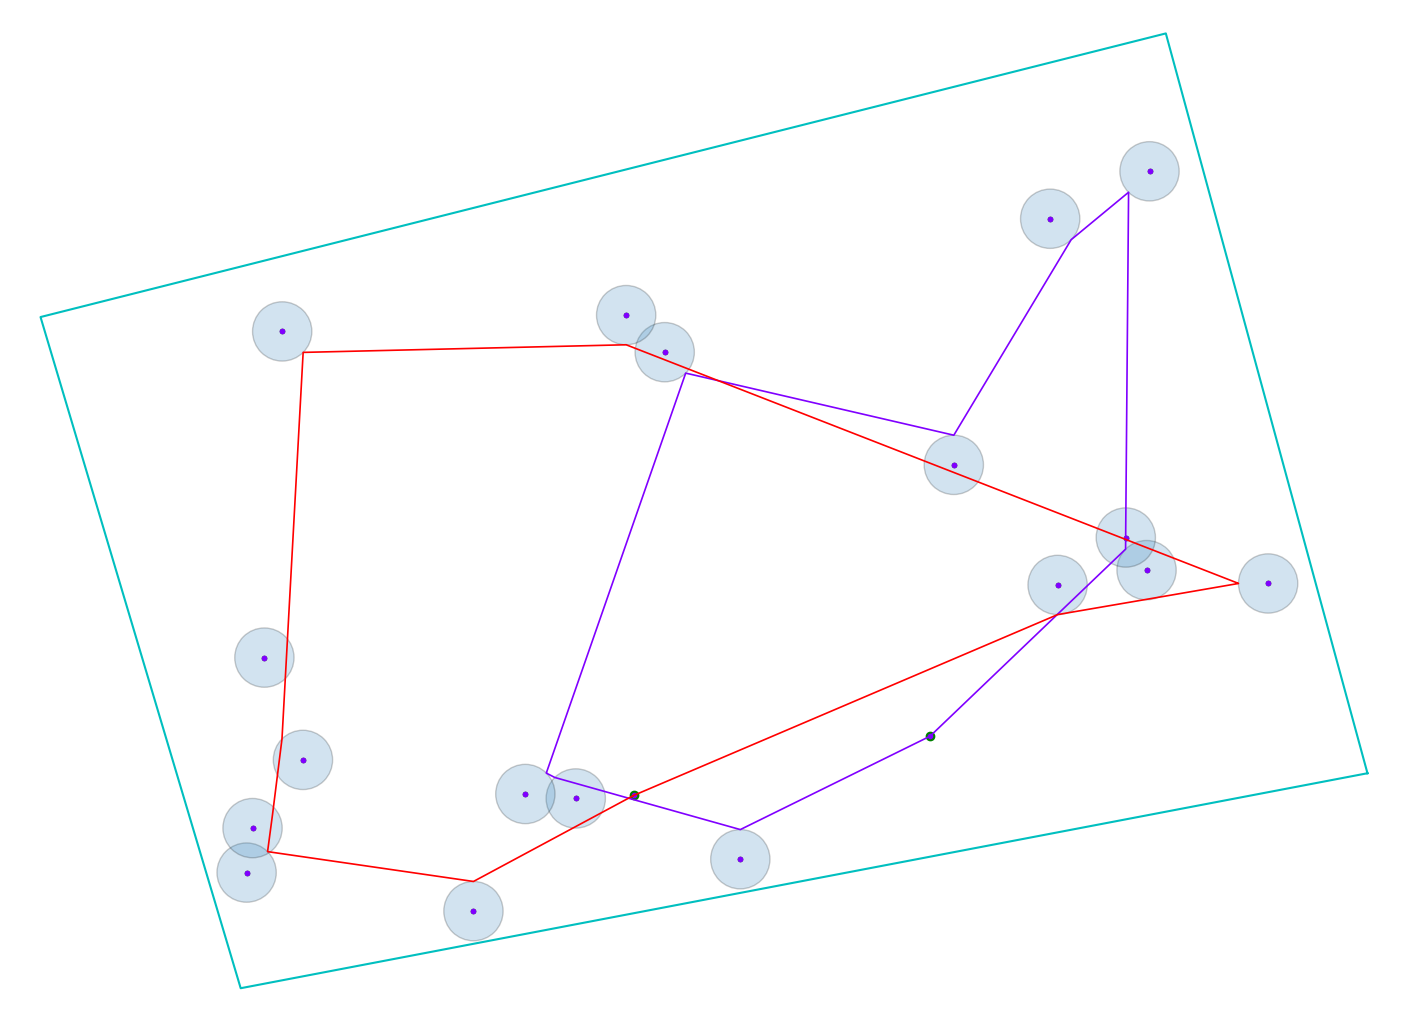
\includegraphics[width=0.8\textwidth]{fig/tsp_segments.png}
    \end{figure}

  \end{frame}
  %%}

  %%{ Sampled segments
  \begin{frame}
    \frametitle{Sampling segments for the UAV's tracker}

    \begin{figure}
      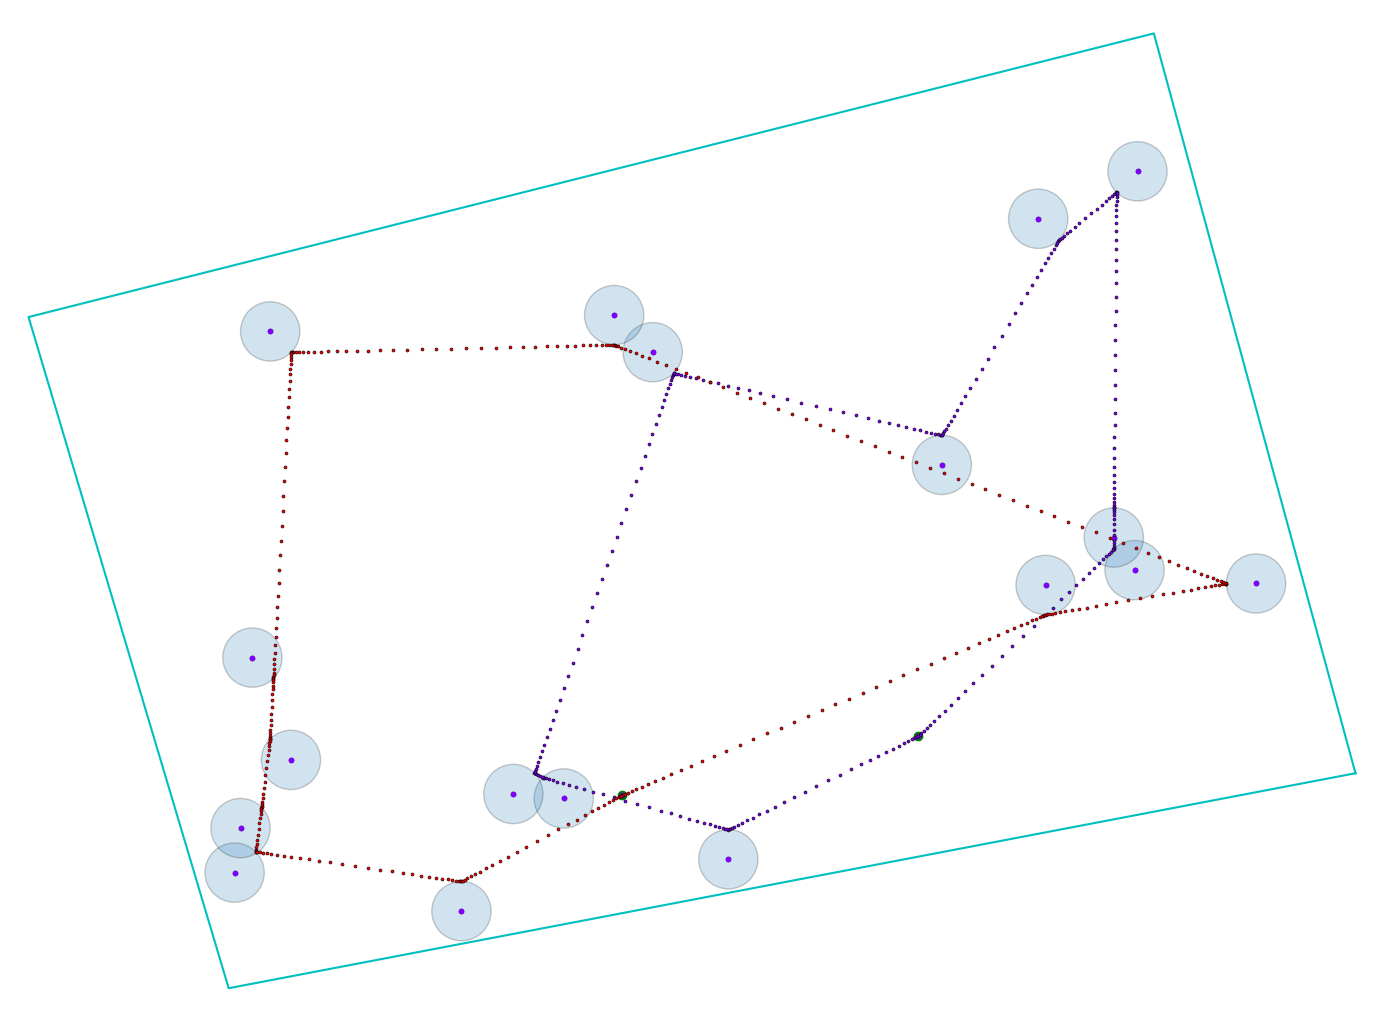
\includegraphics[width=0.8\textwidth]{fig/tsp_segments_sampled.png}
    \end{figure}

  \end{frame}
  %%}

  %%{ With Dubins
  \begin{frame}
    \frametitle{Using the Dubins vehicle model}

    \begin{figure}
      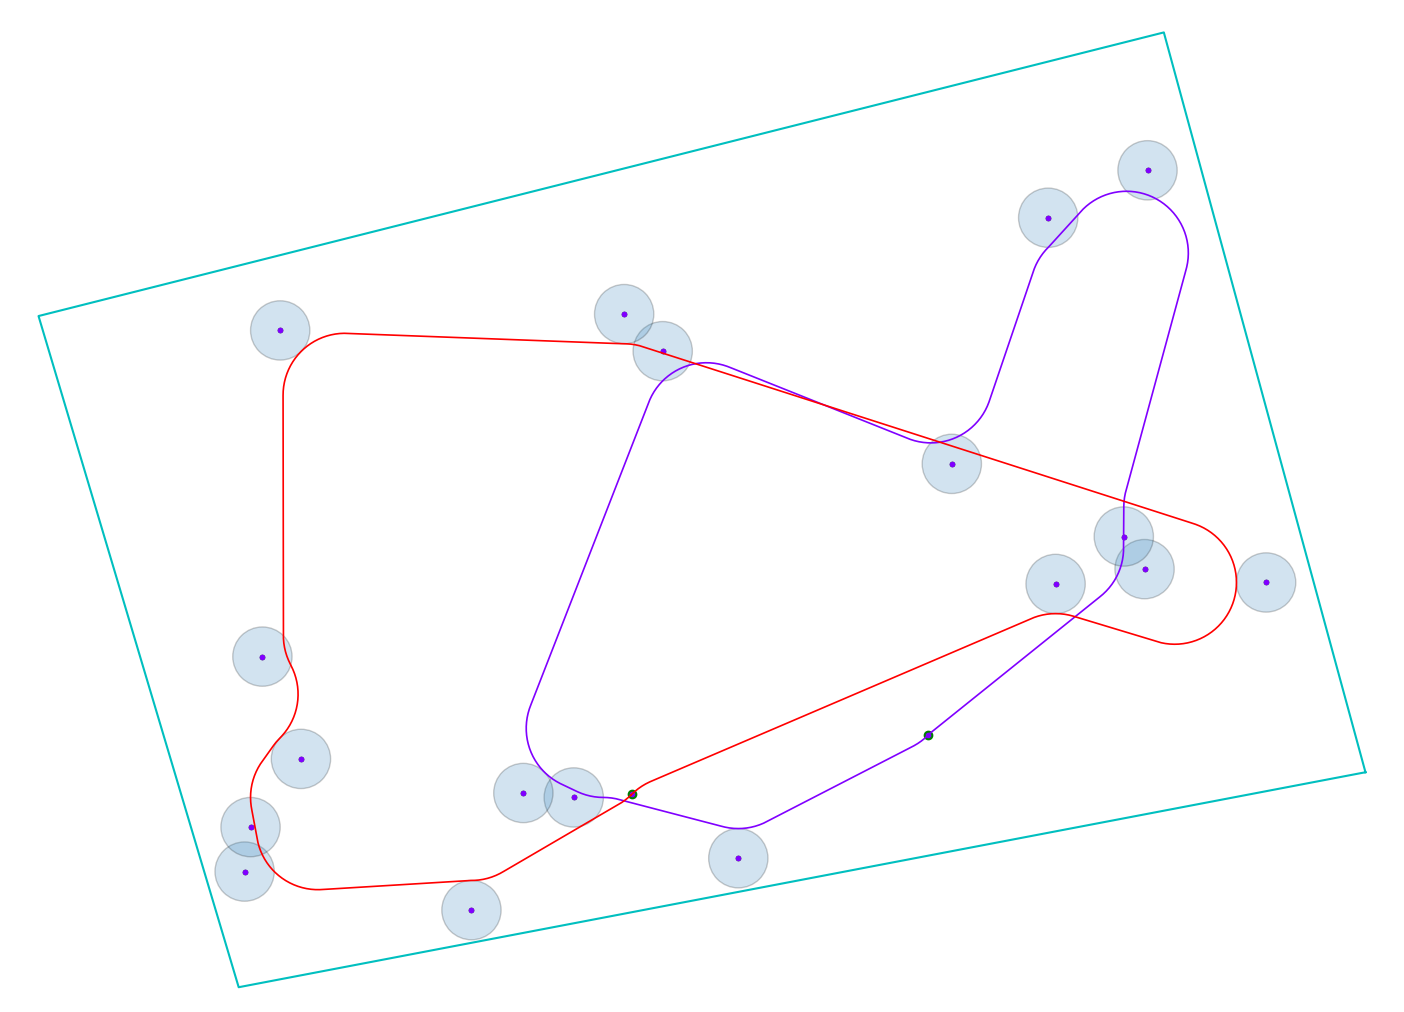
\includegraphics[width=0.8\textwidth]{fig/tsp_dubins.png}
    \end{figure}

  \end{frame}
  %%}

  %%{ Sampling the Dubins path
  \begin{frame}
    \frametitle{Sampling the path for the UAV's tracker}

    \begin{figure}
      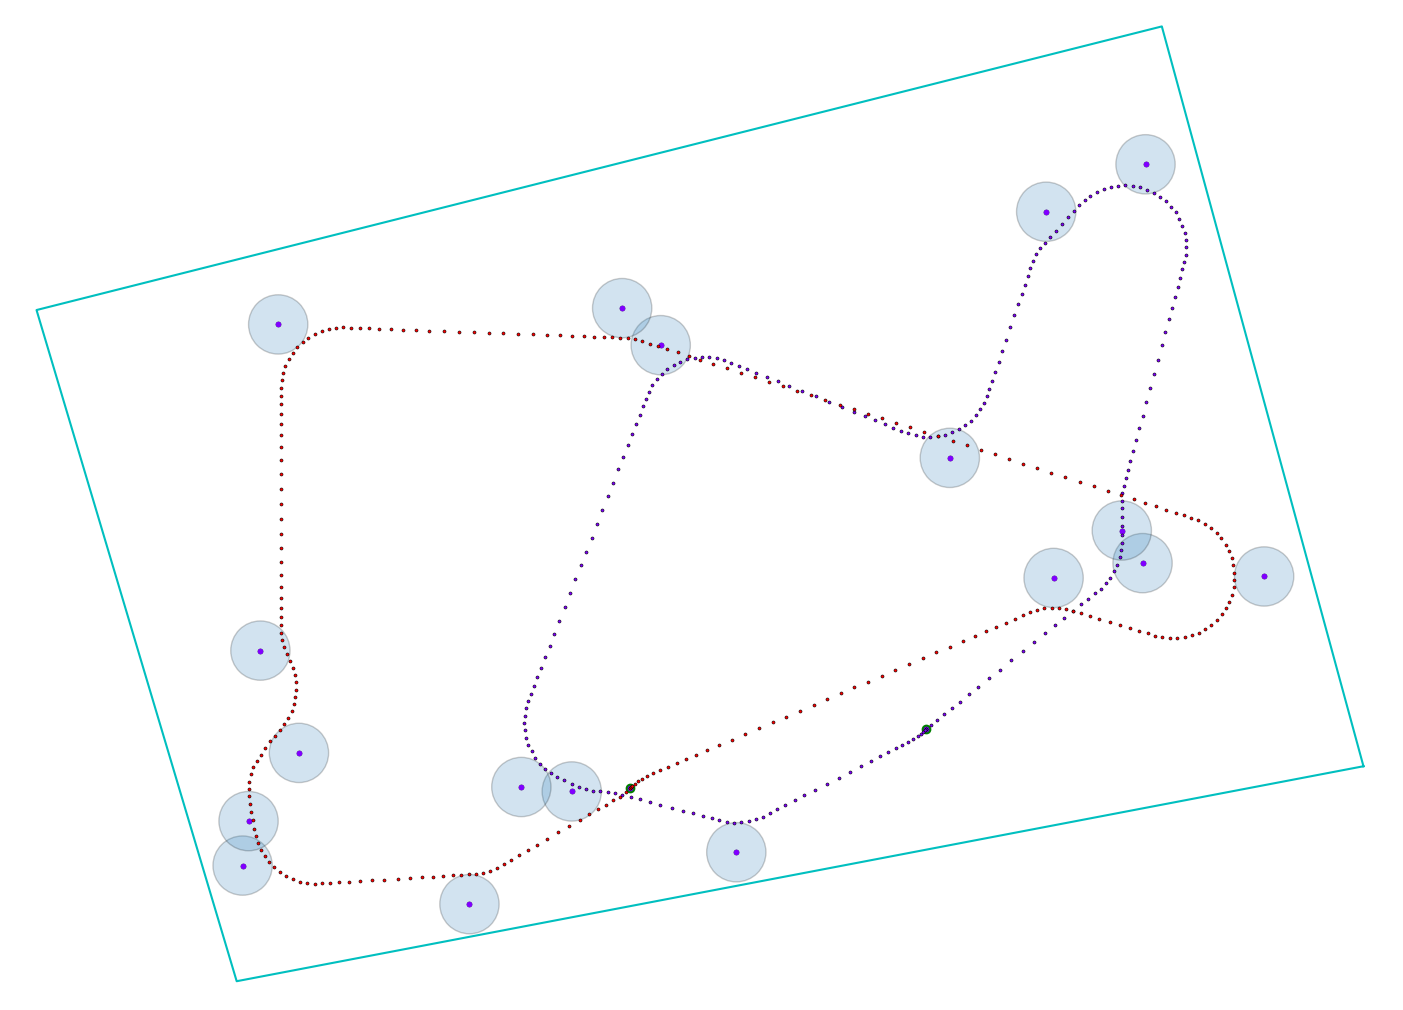
\includegraphics[width=0.8\textwidth]{fig/tsp_dubins_sampled.png}
    \end{figure}

  \end{frame}
  %%}

  %%{ Show the live demo
  \begin{frame}
    \frametitle{Show the live demo}

    \begin{center}
      \large Now is the time to show the Live demo.\\
      \vspace{2em}
      Message to future me: ``How did the last one go? ;-)''
    \end{center}

  \end{frame}
  %%}

  \subsection{running the simulation}

  %%{ Plotting the trajectory in RVIZ

  \begin{frame}
    \frametitle{Plotting the trajectory in RVIZ}

    \begin{figure}
      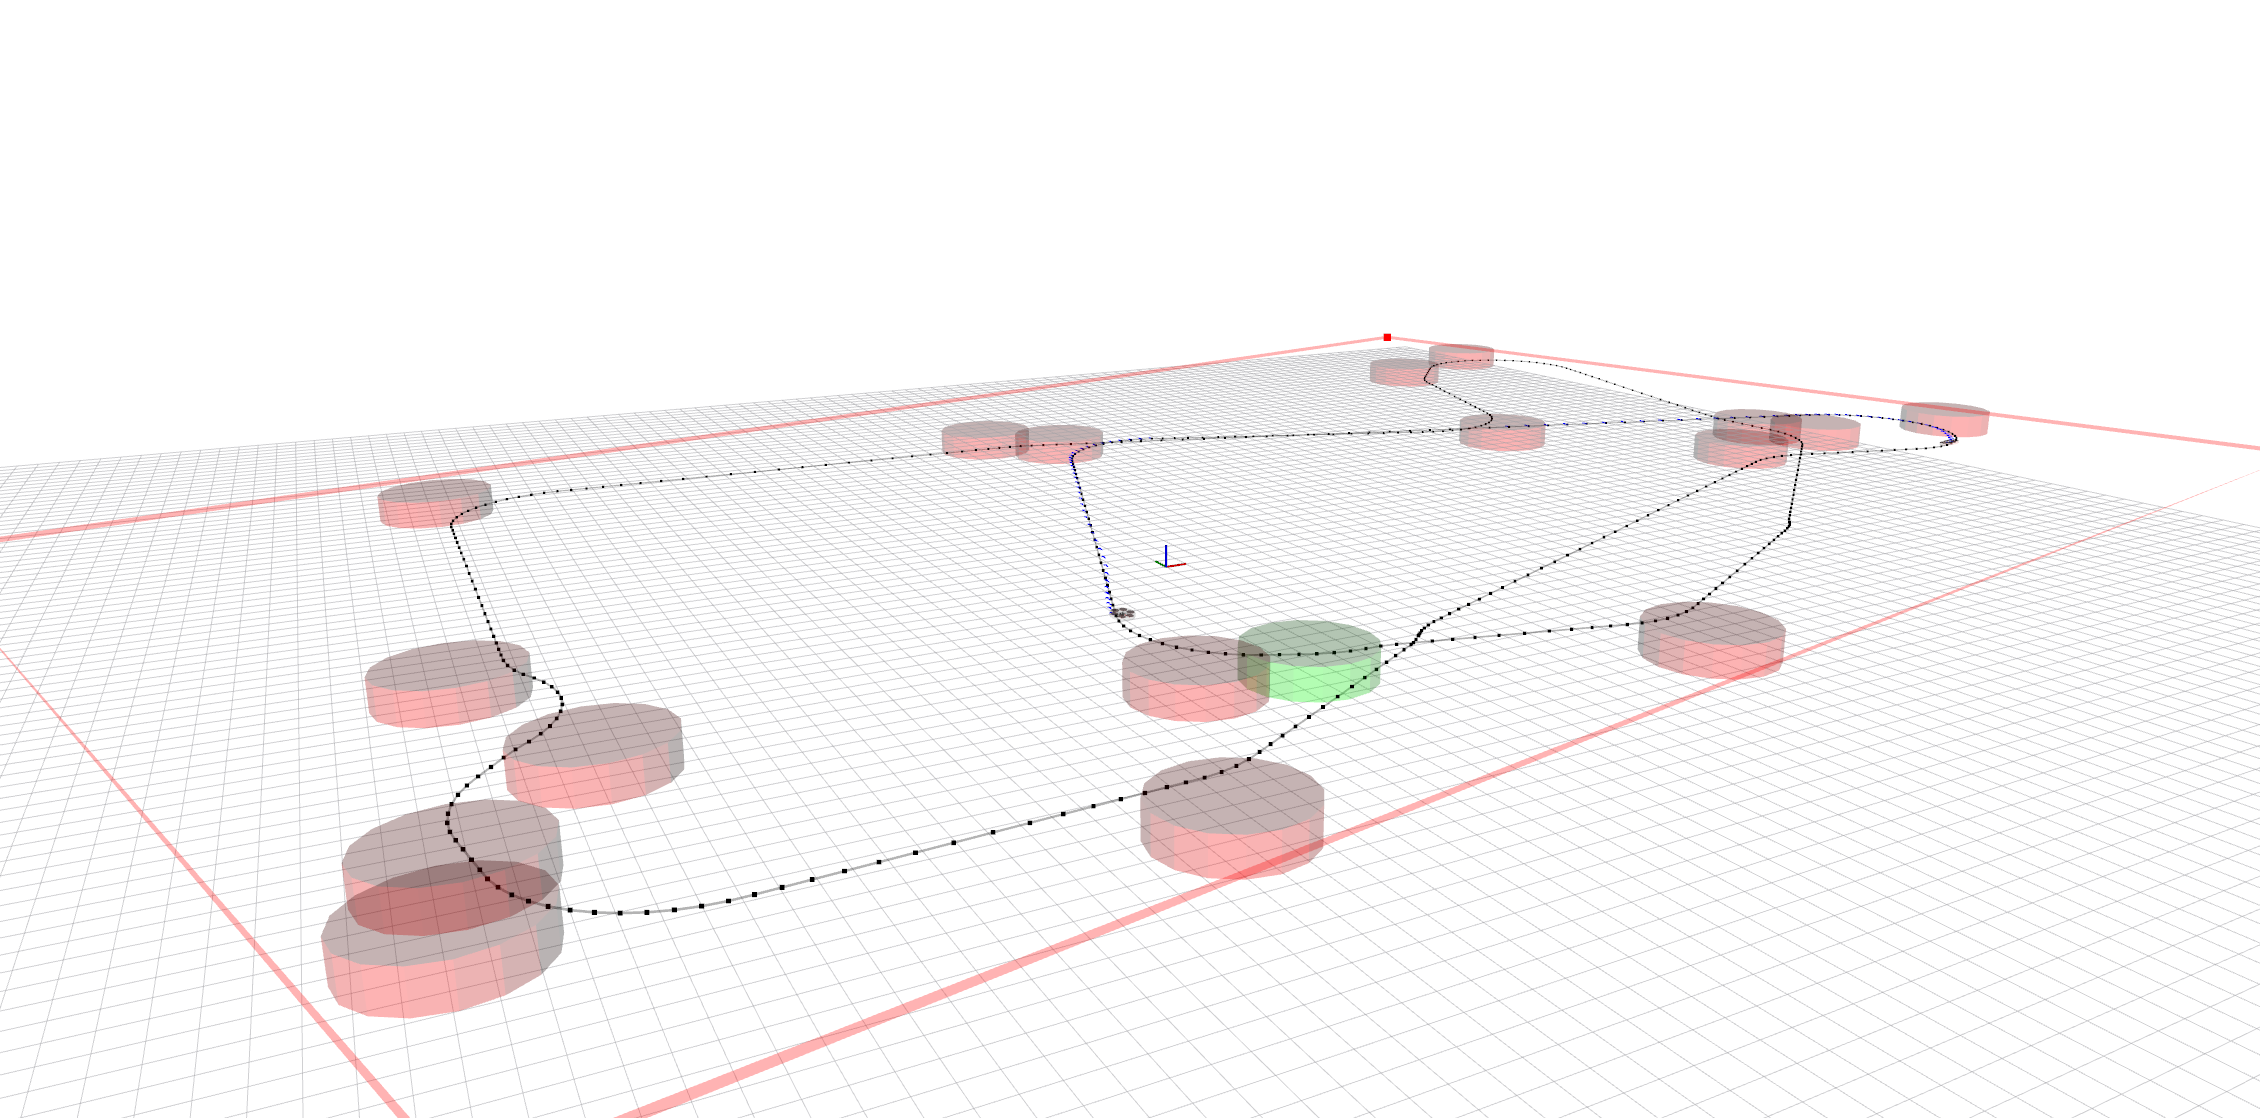
\includegraphics[width=1.0\textwidth]{fig/rviz_1.png}
    \end{figure}

  \end{frame}

  %%}

  %%{ Showing Results in RVIZ

  \begin{frame}
    \frametitle{Showing Results in RVIZ}

    \begin{figure}
      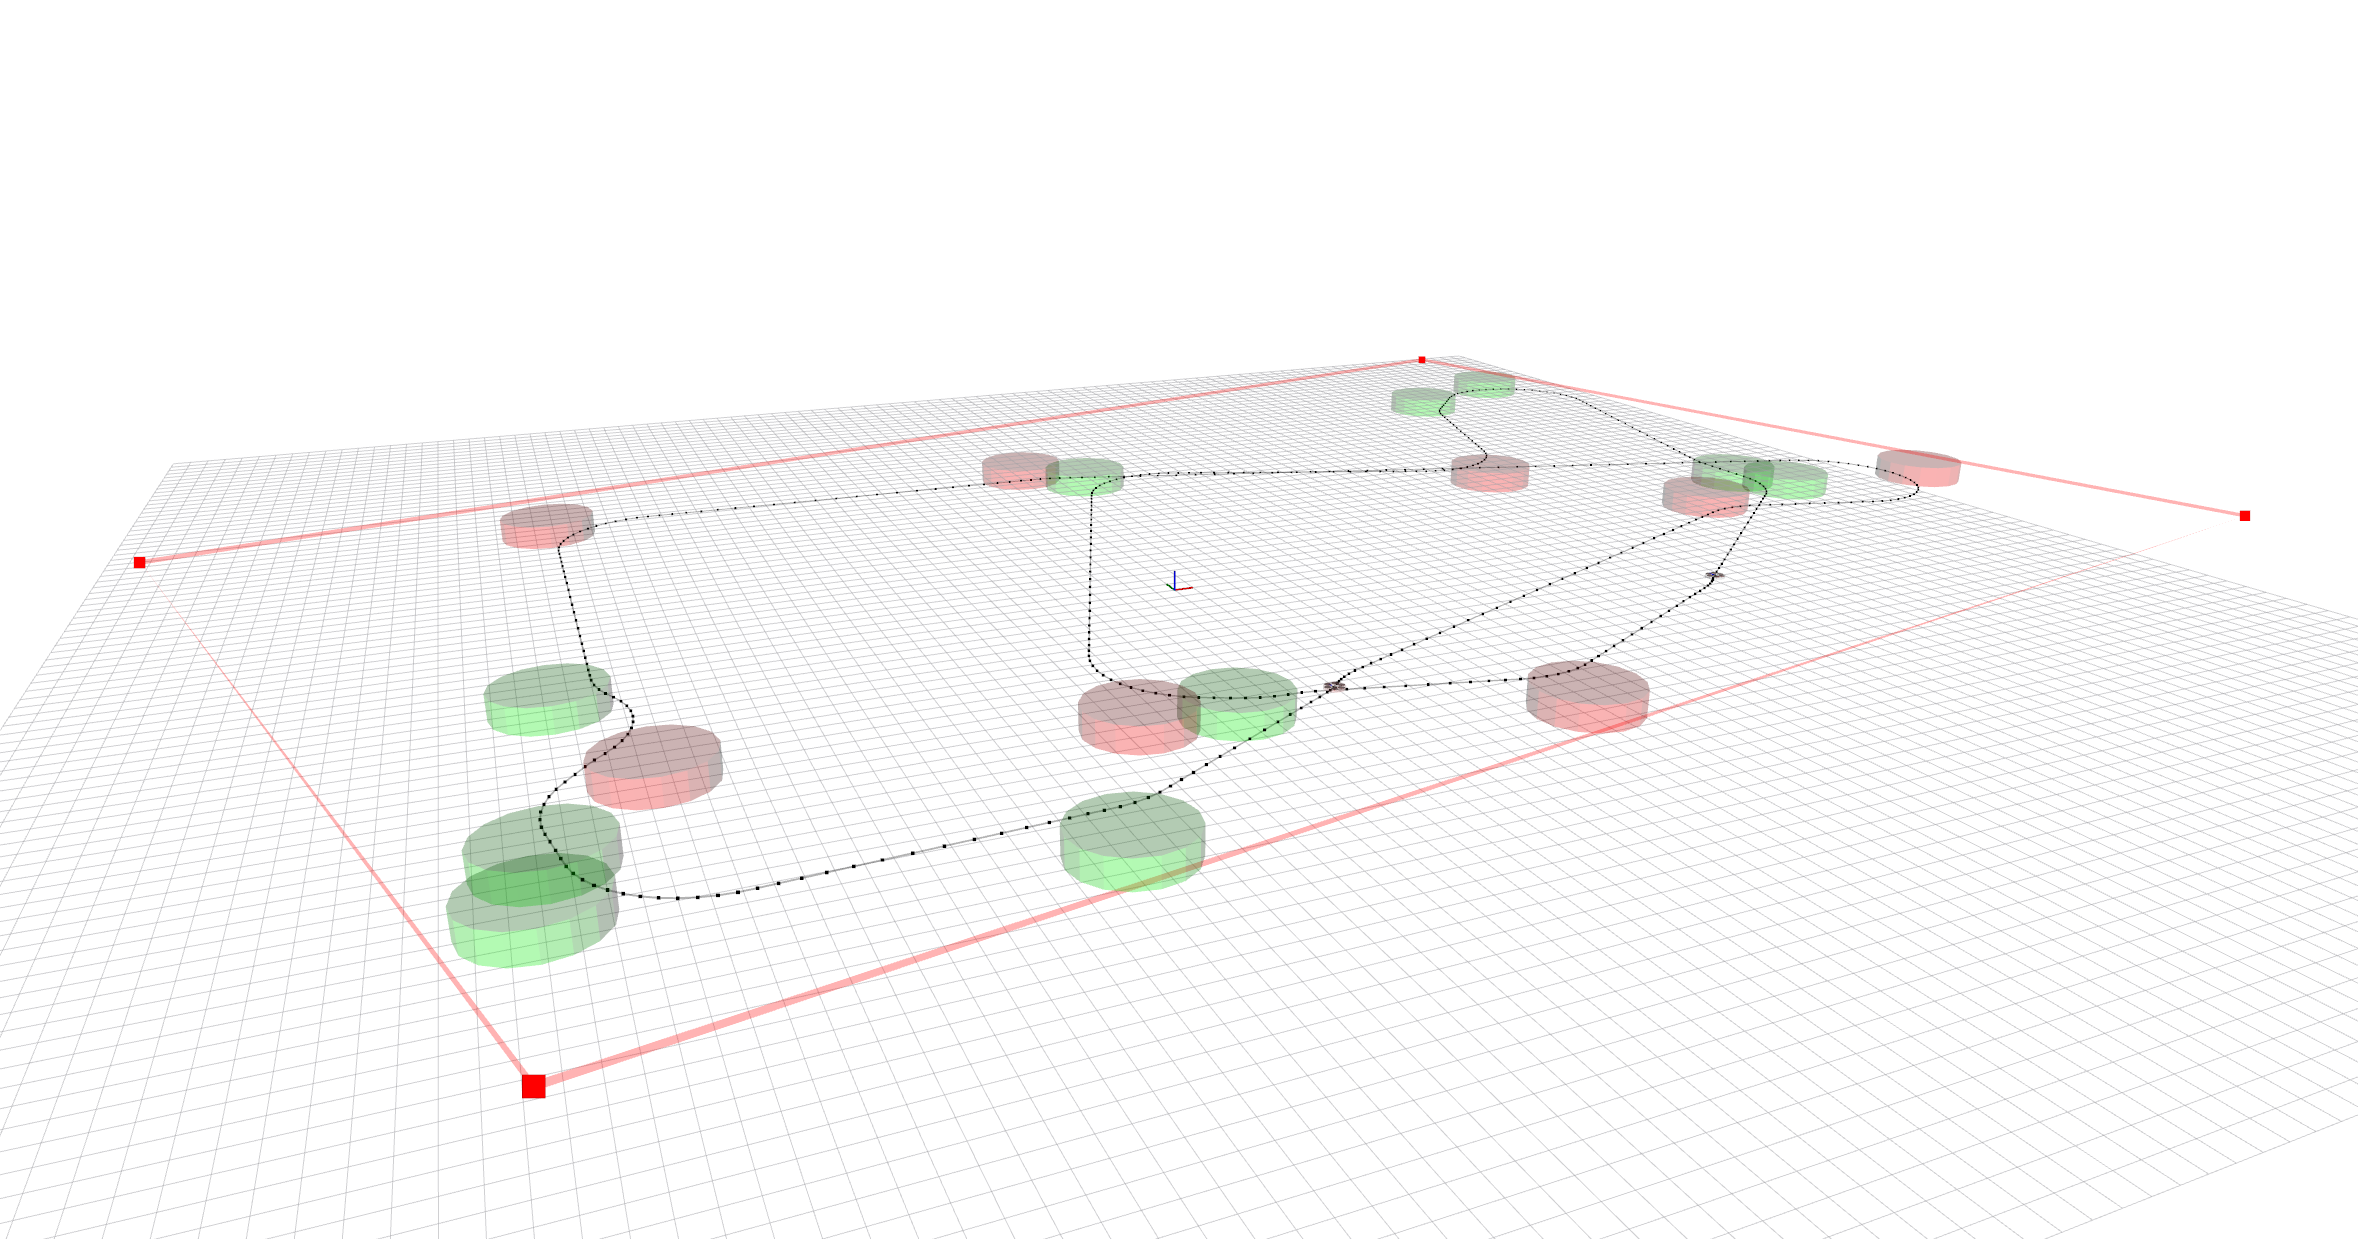
\includegraphics[width=1.0\textwidth]{fig/rviz_2.png}
    \end{figure}

  \end{frame}

  %%}

  %% --------------------------------------------------------------
  %% |                          Resources                         |
  %% --------------------------------------------------------------

  %%{ MRS wiki

  \begin{frame}
    \frametitle{MRS UAV System wiki}
    \begin{figure}
      \vspace{-1em}
      \caption*{\url{http://ctu-mrs.github.io}}
      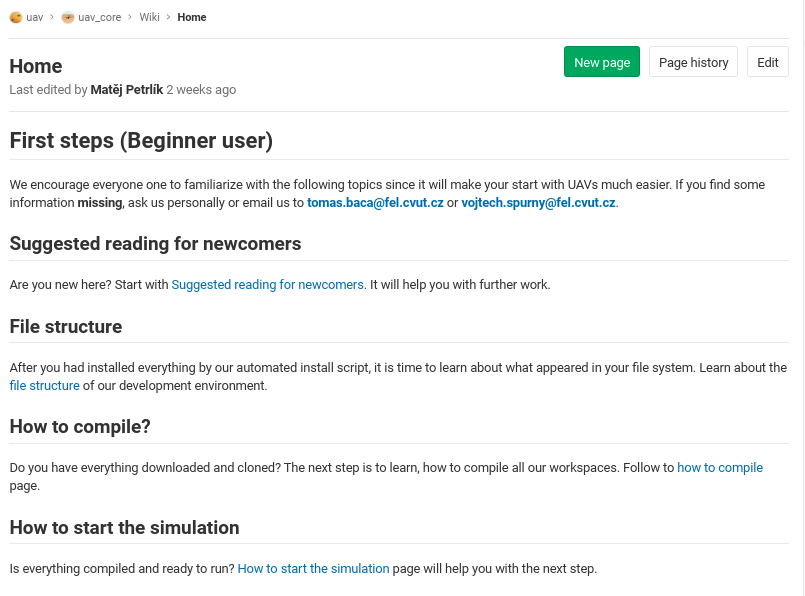
\includegraphics[width=0.7\textwidth]{fig/wiki.png}
    \end{figure}

  \end{frame}

  %%}

  %%{ MRS Cheat Sheet

  \begin{frame}
    \frametitle{The MRS Cheat Sheet}
    \vspace{-1.0em}
    \begin{figure}
      \caption*{\url{http://github.com/ctu-mrs/mrs_cheatsheet}}
      \vspace{-0.5em}
      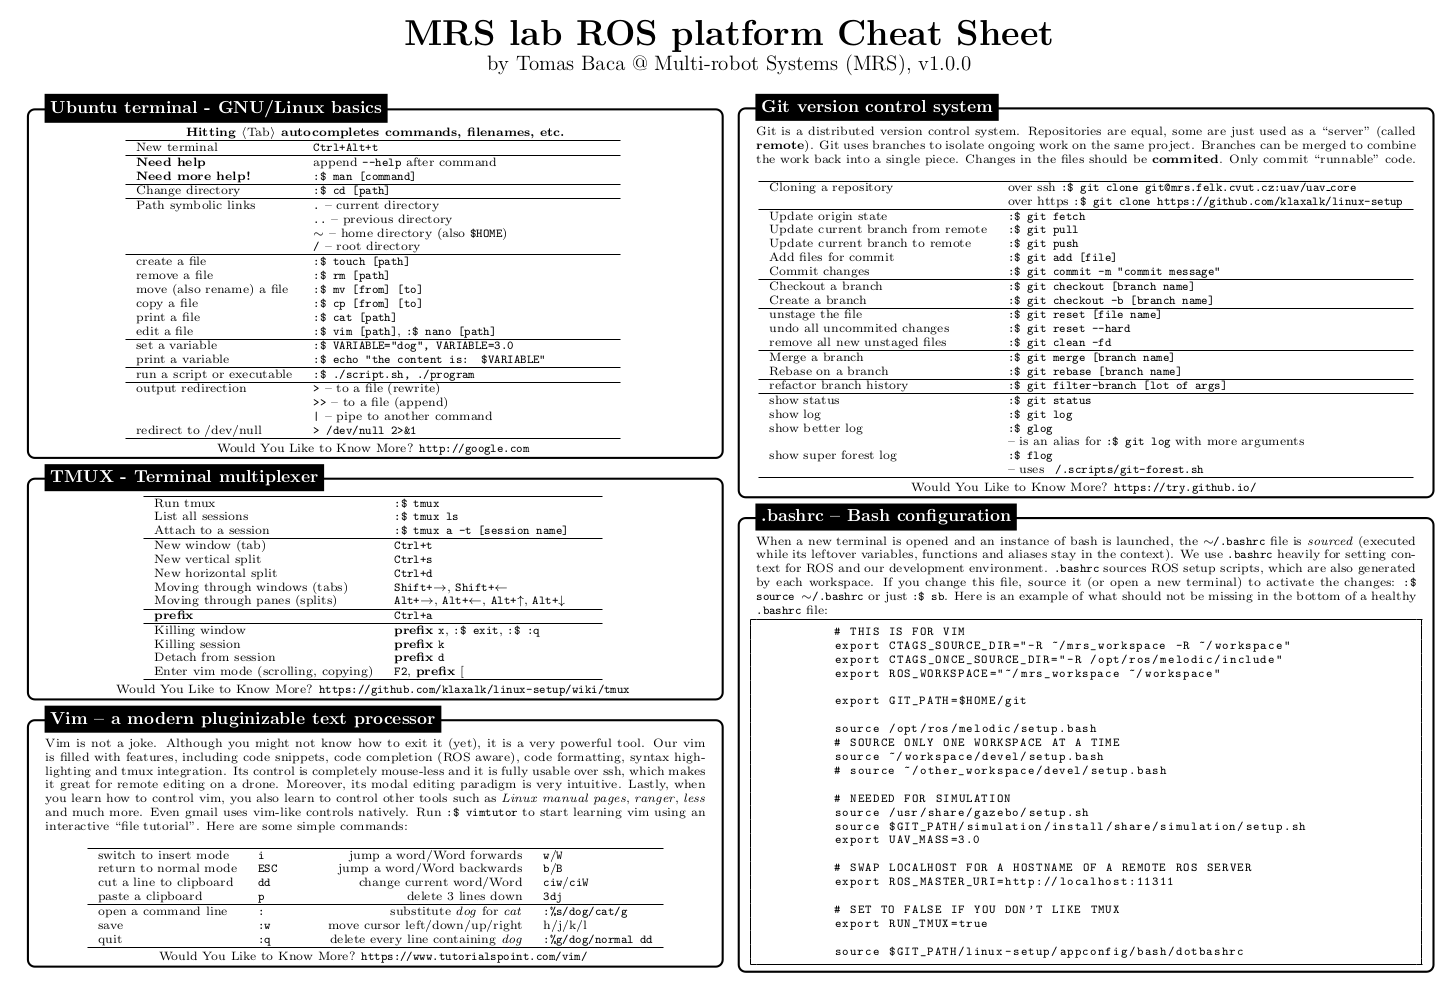
\includegraphics[width=0.8\textwidth]{fig/mrs_cheatsheet.png}
    \end{figure}

  \end{frame}

  %%}

  %%{ Links
  \begin{frame}
    \frametitle{Links}

    \begin{tabular}{ll}

      MRS UAV System & {\small \url{github.com/mrs_uav_system}}\\
      MRS UAV System wiki                       & {\small \url{ctu-mrs.github.io}}\\
      MRS cheat sheet                & {\small \url{github.com/ctu-mrs/mrs_cheatsheet}}\\
      Summer School Seminar Task \#1 & {\small \url{github.com/ctu-mrs/uvdar_leader_follower}}\\
      Summer School Seminar Task \#2 & {\small \url{github.com/ctu-mrs/mtsp_planning_task}}\\
      This presentation              & {\small \url{github.com/ctu-mrs/summer_school_presentation}}\\
      Tomas's Linux setup Repository & {\small \url{github.com/klaxalk/linux-setup}}\\
    \end{tabular}

  \end{frame}
  %%}

  %%{ REFERENCES

  \begin{frame}
    \frametitle{References}
    \tiny{
      \begin{thebibliography}{99}

        \bibitem[Baca et al., 2016]{baca2016embedded} Baca, T and Loianno, G and Saska, M
          \newblock Embedded Model Predictive Control of Unmanned Micro Aerial Vehicles
          \newblock 2016 IEEE International Conference on Methods and Models in Automation in Robotics

        \bibitem[Chudoba et al., 2016]{chudoba2016exploration} Chudoba, J and Kulish, M and Saska, M and Baca, T and Preucil, L
          \newblock Exploration and Mapping Technique Suited for Visual-features Based Localization of MAVs
          \newblock Journal of Intelligent Robotics Systems, 2016


        \bibitem[Spurny et al., 2016]{spurny2016complex} Spurny, V and Baca, T and Saska, M
          \newblock Complex manoeuvres of heterogeneous MAV-UGV formations using a model predictive control
          \newblock 2016 IEEE International Conference on Methods and Models in Automation in Robotics

        \bibitem[Saska et al, 2016]{saska2016auro} Saska, M and Baca, T and Thomas, J and Chudoba, J and Preucil, L and Krajnik, T and Faigl, J and Loianno, G and Kumar, V
          \newblock System for deployment of groups of unmanned micro aerial vehicles in GPS-denied environments using onboard visual relative localization
          \newblock Autonomous Robots, 2016

        \bibitem[Baca et al., 2018]{baca2018model} Baca, T and Hert, D and Loianno, G and Saska, M and Kumar, V
          \newblock Model Predictive Trajectory Tracking and Collision Avoidance for Reliable Outdoor Deployment of Unmanned Aerial Vehicles
          \newblock 2018 IEEE/RSJ International Conference on Intelligent Robots and Systems

        \bibitem[Baca et al., 2020, arXiv:2008.08050]{baca2020mrs} Baca, T and Petrlik, M and Vrba, M and Spurny, V and Penicka, R and Hert, D and Saska, M
          \newblock The MRS UAV System: Pushing the Frontiers of Reproducible Research, Real-world Deployment, and Education with Autonomous Unmanned Aerial Vehicles
          \newblock \url{http://arxiv.org/abs/2008.08050}


      \end{thebibliography}
    }
  \end{frame}

  %%}

\end{document}
